\documentclass[final]{cpecmu}

%% This is a sample document demonstrating how to use the CPECMU
%% project template. If you are having trouble, see "cpecmu.pdf" for
%% documentation.

\projectNo{P804-2}
\acadyear{2022}

\titleTH{ ระบบการยืนยันตัวตนด้วยการใช้ภาพใบหน้าเพื่อเข้าสู่สถานที่ด้วยการใช้กลวิธีการเรียนรู้ของเครื่องแบบต่อเนื่อง}
\titleEN{Facial authentication system for building access using adaptive machine learning technique}

\author{นายนฤสรณ์ กันจินะ}{Naruson Kanchina}{620612153}

\cpeadvisor{paskorn}
\cpecommittee{kampol}
\cpecommittee{natthanan}

%% Some possible packages to include:
\usepackage[final]{graphicx} % for including graphics

%% Add bookmarks and hyperlinks in the document.
\PassOptionsToPackage{hyphens}{url}
\usepackage[colorlinks=true,allcolors=Blue4,citecolor=red,linktoc=all]{hyperref}
\def\UrlLeft#1\UrlRight{$#1$}

%% Needed just by this example, but maybe not by most reports
\usepackage{afterpage} % for outputting
\usepackage{pdflscape} % for landscape figures and tables. 

%% Some other useful packages. Look these up to find out how to use
%% them.
% \usepackage{natbib}    % for author-year citation styles
% \usepackage{txfonts}
% \usepackage{appendix}  % for appendices on a per-chapter basis
% \usepackage{xtab}      % for tables that go over multiple pages
% \usepackage{subfigure} % for subfigures within a figure
% \usepackage{pstricks,pdftricks} % for access to special PostScript and PDF commands
% \usepackage{nomencl}   % if you have a list of abbreviations

%% if you're having problems with overfull boxes, you may need to increase
%% the tolerance to 9999
% \tolerance=9999

\bibliographystyle{plain}
% \bibliographystyle{IEEEbib}

% \renewcommand{\topfraction}{0.85}
% \renewcommand{\textfraction}{0.1}
% \renewcommand{\floatpagefraction}{0.75}

%% Example for glossary entry
%% Need to use glossary option
%% See glossaries package for complete documentation.
\ifglossary
  \newglossaryentry{lorem ipsum}{
    name=lorem ipsum,
    description={derived from Latin dolorem ipsum, translated as ``pain itself''}
  }
\fi

%% Uncomment this command to preview only specified LaTeX file(s)
%% imported with \include command below.
%% Any other file imported via \include but not specified here will not
%% be previewed.
%% Useful if your report is large, as you might not want to build
%% the entire file when editing a certain part of your report.
% \includeonly{chapters/intro,chapters/background}

\begin{document}
\maketitle
\makesignature

\ifproject
\begin{abstractTH}
% เขียนบทคัดย่อของโครงงานที่นี่

% การเขียนรายงานเป็นส่วนหนึ่งของการทำโครงงานวิศวกรรมคอมพิวเตอร์
% เพื่อทบทวนทฤษฎีที่เกี่ยวข้อง อธิบายขั้นตอนวิธีแก้ปัญหาเชิงวิศวกรรม และวิเคราะห์และสรุปผลการทดลองอุปกรณ์ และระบบต่าง ๆ
% \enskip อย่างไรก็ดี การสร้างรูปเล่มรายงานให้ถูกรูปแบบนั้นเป็นขั้นตอนที่ยุ่งยาก
% แม้ว่าจะมีต้นแบบสำหรับใช้ในโปรแกรม Microsoft Word แล้วก็ตาม
% แต่นักศึกษาส่วนใหญ่ยังคงค้นพบว่าการใช้งานมีความซับซ้อน และเกิดความผิดพลาดในการจัดรูปแบบ กำหนดเลขหัวข้อ และสร้างสารบัญอยู่
% \enskip ภาควิชาวิศวกรรมคอมพิวเตอร์จึงได้จัดทำต้นแบบรูปเล่มรายงานโดยใช้ระบบจัดเตรียมเอกสาร
% \LaTeX{} เพื่อช่วยให้นักศึกษาเขียนรายงานได้อย่างสะดวกและรวดเร็วมากยิ่งขึ้น

การระบุตัวตนด้วยการใช้รูปภาพใบหน้าบุคคลเพื่อเข้าสู่สถานที่เป็นหนึ่งในรูปแบบการยืนยันตัวตนที่ช่วยลดการแพร่ระบาดของโรคติดเชื้อไวรัสโคโรนา (COVID-19)
การใช้รูปภาพใบหน้าบุคคลนั้นยังมีจุดอ่อนเมื่อใบหน้าบุคคลมีการเปลี่ยนแปลง เช่น หนวดเครายาวขึ้น สวมแว่นตา เป็นต้น จึงมีการใช้กลวิธีการเรียนรู้แบบต่อเนื่องเพื่อนำรูปภาพใบหน้าใหม่ไปทำการเรียนรู้
เพื่อลดจุดอ่อนของการใช้รูปภาพใบหน้าบุคคล ทางเข้าสถานที่นั้นมีพื้นที่ในการติดตั้งน้อยในโครงงานนี้จึงเลือกใช้ Raspberry Pi และในโปรเจกต์นี้ได้ทำการติดตั้งที่ทางเข้าห้องแลป OASYS 
เนื่องจาก Raspberry Pi นั้นมีประสิทธิภาพไม่เพียงพอต่อการระบุตัวตน หรือ การเรียนรูปรูปภาพใบหน้าบุคคล ในโปรเจกต์นี้จึงใช้ Raspberry Pi ทำหน้าที่ตรวจจับใบหน้า และใช้เซิร์ฟเวอร์ในการระบุตัวตน 
และเรียนรู้รูปภาพใบหน้าบุคคล โดยแบบจำลองการตรวจจับใบหน้าบน Raspberry Pi นั้นสามารถที่จะตรวจจับใบหน้าบุคคลได้ดี ซึ่งเวลาเฉลี่ยในการแสดงผลการระบุตัวตนหลังจากการตรวจจับใบหน้านั้นน้อยกว่า 500 มิลลิวินาที 
และยังมีการยืนยันตัวตนด้วยรหัสอีกขึ้นตอนเพื่อลดความผิดพลาดในการระบุตัวตน ทำให้ผู้ใช้งานยังได้รับความสะดวก ปลอดภัยจากโรคติดเชื้อไวรัสโคโรนา (COVID-19) จากการใช้งาน และยังมีความแม่นยำ

\end{abstractTH}

\begin{abstract}
% The abstract would be placed here. It usually does not exceed 350 words
% long (not counting the heading), and must not take up more than one (1) page
% (even if fewer than 350 words long).

% Make sure your abstract sits inside the \texttt{abstract} environment.

Using facial recognition technology to identify individuals and grant access to a location is one form of identity verification 
that helps reduce the spread of COVID-19. However, using facial images has its weaknesses when a person's face changes, such as 
growing a beard or wearing glasses. Therefore, continuous learning algorithms are used to improve the accuracy of new facial images. 
Due to limited space, the Raspberry Pi was chosen for this project, and it was installed at the entrance of the OASYS lab. Raspberry Pi's 
performance is insufficient for facial recognition and learning images, so in this project, it was used to detect faces, and a server was used 
for identity verification and image learning. The facial detection model on the Raspberry Pi works well and takes less than 500 milliseconds on 
average to verify identity after detecting a face. Additionally, there is a confirmation process to reduce the likelihood of identity errors, which 
makes it convenient and safe for users to use and helps prevent the spread of COVID-19.


\end{abstract}

\iffalse
\begin{dedication}
This document is dedicated to all Chiang Mai University students.

Dedication page is optional.
\end{dedication}
\fi % \iffalse

\begin{acknowledgments}
\indent โครงงานนี้จะไม่สำเร็จลุล่วงลงได้ ถ้าไม่ได้รับความกรุณาจาก ผศ.ดร.ภาสกร แช่มประเสริฐ
อาจารย์ที่ปรึกษา ที่ได้สละเวลาให้ความช่วยเหลือทั้งให้คำแนะนำ ให้ความรู้และแนวคิดต่าง ๆ รวมถึง
อ.ดร.\,ณัฐนันท์ พรหมสุข และ ผศ.ดร.กำพล วรดิษฐ์ ที่ให้คำปรึกษาจนทำให้โครงงานเล่มนี้เสร็จ
สมบูรณ์ไปได้ \\
\indent ขอบคุณห้องวิจัย OASYS ภาควิชาวิศวกรรมคอมพิวเตอร์ คณะวิศวกรรมศาสตร์
มหาวิทยาลัยเชียงใหม่ ที่เอื้อเฟื้อสถานที่ในการทำโครงงาน สนับสนุนอุปกรณ์ต่าง ๆ และ
ขอขอบคุณ นาย กมลพัฒน์ สุนทรพงศ์ และ นางสาวโชติโรส ประถม ที่คอยให้ความช่วยเหลือในการทำโครงงานมาโดยตลอด \\
\indent ขอขอบคุณทาง ITSC ที่ได้ให้ใช้เซิร์ฟเวอร์ และขอบคุณเพื่อน ๆ ที่ให้กำลังใจรวมถึงคำแนะนำที่ดีตลอดการทำโครงงานที่ผ่านมา 
รวมทั้งขอขอบพระคุณอีกหลาย ๆ ท่านที่ไม่ได้เอ่ยนามมา ณ ที่นี้ ที่ได้ให้ความ
ช่วยเหลือตลอดมา หากหนังสือโครงงานเล่มนี้มีข้อผิดพลาดประการใด กระผมขอน้อมรับด้วยความ
ยินดี


% \texttt{acknowledgment} environment.

\acksign{2022}{12}{12}
\end{acknowledgments}%
\fi % \ifproject

\contentspage

\ifproject
% \figurelistpage

% \tablelistpage
\fi % \ifproject

% \abbrlist % this page is optional

% \symlist % this page is optional

% \preface % this section is optional


\pagestyle{empty}\cleardoublepage
\normalspacing \setcounter{page}{1} \pagenumbering{arabic} \pagestyle{cpecmu}

\chapter{\ifenglish Introduction\else บทนำ\fi}

\section{\ifenglish Project rationale\else ที่มาของโครงงาน\fi}
การยืนยันตัวตนในการเข้าสถานที่หลายรูปแบบ เช่น การแสกนลายนิ้วมือ การใช้บัตรประจำตัว  การระบุเอกลักษณ์ด้วยคลื่นวิทยุ (Radio Frequency Identification: RFID) และอื่น ๆ อีกมากมาย 
ในปัจจุบันมีสถานการณ์โควิด-19 ยังมีการแพร่ระบาด ทำให้ผู้คนไม่สามารถพบปะระหว่างพนักงานต้อนรับกับผู้ที่เข้าสู่สถานที่ และการสัมผัสกับอุปกรณ์ยืนยันตัวตนทำให้เกิดการแพร่กระจากของโรค 
ส่งผลให้การยืนยันตัวตนในการเข้าสถานที่โดยใช้รูปถ่ายใบหน้าจะช่วยลดการแพร่ระบาดของเชื้อโรค และมีความสะดวกในการใช้งานไม่ต่างกับการยืนยันตัวตนแบบอื่น แต่เมื่อใบหน้าของบุคคลมีการเปลี่ยนแปลงตลอดในทุกวัน 
เช่น มีหนวด ไม่มีหนวด ผมสั้น ผมยาว ใส่แว่น ไม่ใส่แว่น มีผลทำให้การระบุตัวตนด้วยการใช้ภาพใบหน้าจะเกิดความผิดพลาด ซึ่งเป็นปัญหาหลักของการระบุตัวตนด้วยการใช้ภาพใบหน้า
ในสถาณะการณ์ปัจจุบันเกิดวิกฤติขาดแคลนชิปส่งผลให้อุปกรณ์อิเล็กทรอนิกส์มีราคาสูงขึ้น และทางเข้าสถานที่มีพื้นที่จำกัด
% จึงเกิดเป็นที่มาของโครงงานนี้ โดยมีการออกแบบอุปกรณการนำรูปภาพใบหน้าที่ได้รับเข้ามาใหม่ในแต่ละครั้งของการระบุตัวตนนั้น 
% ไปทำการเรียนรู้ใบหน้าใหม่ ทำให้ระบบสามารถจดจำภาพใบหน้าใหม่ที่มีการเปลี่ยนแปลง 
% และความแม่นยำในการระบุตัวตนจะสูงขึ้นเมื่อมีจำนวนรูปภาพใบหน้าที่เก็บไว้มากขึ้น และหลายหลายรูปแบบ ส่งผลให้สามารถแก้ปัญหาของการเปลี่ยนแปลงทางใบหน้าได้ 

\indent จึงเป็นที่มาของโครงงาน โดยได้ออกแบบอุปกรณ์ตรวจจับใบหน้า และแสดงผล ให้มีขนาดที่เล็ก น้ำหนักเบา ใช้เวลาในการติดตั้งที่สั้น ใช้พื้นที่ในการติดตั้งที่น้อย และงบประมาณของระบบที่ใช้นั้นไม่สูง 
โดยระบบตรวจจับใบหน้าที่ได้ออกแบบนั้นสามารถที่จะแยกแยะใบหน้ามนุษย์ได้ทั้งการใส่หน้ากากอนามัยหรือไม่ใส่ และออกแบบเซิร์ฟเวอร์ให้ทำหน้าที่ระบุตัวตน และเรียนรู้รูปภาพใบหน้าเพื่อนำไปเป็นแบบจำลองใบหน้าบุคคล 
ซึ่งจะนำรูปภาพใบหน้าที่ได้รับการยืนยันตัวตนในครั้งใหม่ไปทำการเรียนรู้ด้วย เมื่อมีการระบบตัวตนผิดพลาดหรือมีความแม่นยำที่ต่ำกว่าค่าที่กำหนดก็จะมีการใช้รหัสในการระบุตัวตน 
เพื่อเข้ามาช่วยในการยืนยันตัวตนให้มีความปลอดภัยมากยิ่งขึ้น
% โดยเมื่อระบบตัวตนแล้วนั้นผู้ใช้จะสามารถให้คะแนนของการระบุตัวตนเพื่อที่จะเป็นการยืนยันการระบุตัวตนว่ามีความถูกหรือผิด

\section{\ifenglish Objectives\else วัตถุประสงค์ของโครงงาน\fi}
\begin{enumerate}
    \item เพื่อพัฒนาระบบตรวจจับใบหน้ามนุษย์ให้มีความแม่นยำที่สูง
    \item เพื่อให้ระบบมีความเหมาะสมของอุปกรณ์ที่ติดตั้ง
    \item เพื่อให้ระบบสามารถนำไปใช้งานได้จริง
\end{enumerate}

\section{\ifenglish Project scope\else ขอบเขตของโครงงาน\fi}
โดยระบบตรวจจับใบหน้าจะทำการติดตั้งหน้าทางเข้าห้องกลุ่มวิจัยทฤษฎีและการประยุกต์ใช้การหาค่าที่เหมาะสมที่สุดในระบบทางวิศวกรรม 
(OASYS Research Group Optimization Theory and Applications for Engineering SYStems Research Group: OASYS) 
และปรับให้มีความแม่นยำมากที่สุดให้ยังคงความพึงพอใจของผู้ใช้ห้องได้

\subsection{\ifenglish Hardware scope\else ขอบเขตด้านฮาร์ดแวร์\fi}
\begin{enumerate}
    \item ระบบจะสามารถค้นหาใบหน้าได้จะต้องมีพื้นที่ที่มีแสงสว่างเพียงพอ
    \item พื้นที่ที่ทำการติดตั้งต้องมีสัญญานอินเทอร์เน็ตทั้งไร้สายหรือผ่านสายแลน (ข่ายงานบริเวณเฉพาะที่)
    \item พื้นที่ที่ทำการติดตั้งต้องไม่มีผุ้คนพลุกพล่าน
    \item โปรแกรมการเรียนรู้ของเครื่องที่ไม่เกินกําลังด้านฮาร์ดแวร์ของเซิร์ฟเวอร์ที่ใช้เรียนรู้แบบจำลอง (model)
\end{enumerate}

\subsection{\ifenglish Software scope\else ขอบเขตด้านซอฟต์แวร์\fi}
\begin{enumerate}
    \item สามารถจัดเก็บข้อมูลและรูปภาพใบหน้าได้
    \item สามารถที่จะเรียนรู้รูปภาพใหม่ ที่เข้ามาจัดเก็บได้
    \item ระบบใช้เวลาในการตรวจจับใบหน้า ส่งภาพไปหน้าไปยังเซิร์ฟเวอร์ ระบุตัวตน และส่งผลลัพธ์กลับมาแสดงจะให้เวลาไม่เกิน 20 วินาที
\end{enumerate}

\section{\ifenglish Expected outcomes\else ประโยชน์ที่ได้รับ\fi}
\begin{enumerate}
    \item ผู้ที่เข้าสู่สถานที่ลดความเสี่ยงที่จะได้รับเชื่อโรค
    \item ระบบสามารถที่จะระบุตัวตนในเวลาที่น้อย ทำให้ยังคงความสะดวกในการเข้าสู่สถานที่ได้ไม่ต่างจากการเข้าสู่สถานที่รูปแบบอื่น ๆ
    \item ระบบสามารถส่งต่อสัญญานหรือข้อมูลไปยังส่วนอื่น ๆ ได้ เช่น บอกทางไปห้องทำงาน เปิดเครื่องคอมพิวเตอร์ในห้องทำงาน บอกตารางงานของบุคคลนั้น และจดจำเวลาเข้างานหรือออกงาน เป็นต้น
\end{enumerate}

\section{\ifenglish Technology and tools\else เทคโนโลยีและเครื่องมือที่ใช้\fi}
\subsection{\ifenglish Hardware technology\else เทคโนโลยีด้านฮาร์ดแวร์\fi}
\begin{enumerate}
    \item คอมพิวเตอร์ขนาดเล็ก (Raspberry Pi 4 Model B)
    \item กล้องเว็บแคมส์ที่ใช้การเชื่อมต่อผ่านช่องยูเอสบี (บัสคอมพิวเตอร์) (webcam)
    \item จอภาพ (monitor)
    \item แผงแป้นอักขระ (keyboard)
    \item เครื่องบริการ (server)
\end{enumerate}

\subsection{\ifenglish Software technology\else เทคโนโลยีด้านซอฟต์แวร์\fi}
\begin{enumerate}
    \item Python : ภาษาที่ใช้ในการค้นหาภาพใบหน้าบุคคล การส่งรูปภาพใบหน้า และการทำเว็ปเซิร์ฟเวอร์สำหรับรับรูปภาพ
    \item OpenCV : ไลบรารี (Library) ใช้ในการค้นหาใบหน้าบุคคล และใช้ในการระบุตัวตน
    % \item TensorFlow : ไลบรารี (Library) สำหรับการเรียนรู้รูปภาพใบหน้าออกมาเป็นโมเดลโดยสามารถใช้งานได้ดีกับภาษา Python
    \item Tkinter : ไลบรารี (Library) สำหรับการพัฒนา (Graphical User Interface: GUI) ที่ใช้ภาษาไพธอน (Python)
    \item Open Face : โมเดลที่ใช้ในการระบุตันตนบุคคล
    \item MediaPipe : ไลบรารี (Library) ของ (Machine Learning: ML) หรือ (Deep Learning: DL) ที่พัฒนาโดย Google ใช้ในการตรวจจับใบหน้าบุคคล
    \item Flask Framework : เป็นโครงสร้างของ Restful API ที่ใช้ในการทำเว็ปเซิร์ฟเวอร์ที่รับรูปภาพโดยเป็นภาษาไพธอน (Python) ทำให้สามารถเรียกใช้งาน OpenCV หรือ TensorFlow เมื่อรับรูปภาพสำเร็จและส่งผลลัพธ์
    \item Rest API : ใช้ในการสร้างเว็ปเซิร์ฟเวอร์สำหรับรับรูปภาพบนเซิร์ฟเวอร์
    \item Application Programming Interface : ใช้ในการส่งรูปภาพผ่านเอชทีทีพี (HyperText Transfer Protocol: HTTP)
    \item Virtual Studio Code : ใช้ในการพัฒนาการค้นหาใบหน้าแบบเรียลไทม์และทำเว็ปเซิร์ฟเวอร์สำหรับรับรูปภาพ
    
\end{enumerate}

\section{\ifenglish Project plan\else แผนการดำเนินงาน\fi}

\begin{plan}{12}{2021}{3}{2023}
    \planitem{12}{2021}{1}{2022}{ศึกษา และการตรวจจับใบหน้า และการทำงานบน raspbian os และการบีบอัดไฟล์รูปภาพ}
    \planitem{1}{2022}{2}{2022}{ศึกษา และทดลองการส่งรูปภาพผ่าน RESTful API และ Python Flask framework และเทคนิคการปรับรูปภาพ}
    \planitem{3}{2022}{3}{2022}{ศึกษา และทดลองการทำงานของ DNN และการเรียนรู้ภาพใบหน้าบุคคล หรือ Train model }
    \planitem{10}{2022}{11}{2022}{เก็บข้อมูลรูปภาพใบหน้าผู้ใช้งานห้องวิจัย OASYS และออกแบบให้ระบบสามารถตรวจจับใบหน้าได้ดีขึ้น และส่งภาพใบหน้าเร็วขึ้น}
    \planitem{11}{2022}{12}{2022}{ติดตั้ง และทดสอบระบบ และออกแบบและพัฒนาโมเดลการเรียนรู้ภาพใบหน้าบุคคลบนเซิร์ฟเวอร์ และการส่งผลลัพธ์}
    \planitem{12}{2022}{1}{2023}{ออกแบบ และพัฒนา GUI ตอบรับผลลัพธ์ ส่งผลลัพธ์ไปยังเซิร์ฟเวอร์ และเซิร์ฟเวอร์จัดการกับผลลัพธ์ที่ได้รับกลับมา}
    \planitem{1}{2023}{2}{2023}{ทดสอบทั้งระบบ ปรับปรุงระบบ และปรับแต่งระบบให้มีประสิทธิภาพขึ้น}
    \planitem{2}{2023}{3}{2023}{เขียนรายงานสรุปผลการทำงาน}
\end{plan}

\section{\ifenglish Roles and responsibilities\else บทบาทและความรับผิดชอบ\fi}
รับผิดชอบทุกส่วนของโครงงานนี้ โดยที่ต้องใช้ความรู้ด้าน Computer vision, Web service, Storage, \\ Rest API, Machine Learning และพัฒนาการเรียนรู้รูปภาพใบหน้า

\section{\ifenglish%
Impacts of this project on society, health, safety, legal, and cultural issues
\else%
ผลกระทบด้านสังคม สุขภาพ ความปลอดภัย กฎหมาย และวัฒนธรรม
\fi}

สามารถช่วยลดการแพร่ระบาดของเชื้อโควิด-19 ของพนักงานในสถานที่ มีการเก็บรูปภาพบุคคลที่เข้าสถานที่โดยเมื่อมีเหตุการณ์ก็นำรูปที่บันทึกมาใช้เป็นหลักฐานได้โดยรูปภาพใบหน้านั้นจะไม่อนุญาติให้ผู้อื่นนำไปใช้ได้จะสามารถใช้ได้ก็ต่อเมื่อมีการขออณุญาติเรียบร้อยซึ่งจะไม่ขัดกับกฎหมาย 
รูปภาพที่ส่งไปให้เซิร์ฟเวอร์นั้นมีการเข้ารหัสเพื่อป้องกันการโจรกรรมได้ เมื่อยืนยันตัวตนสำเร็จก็สามารถนำข้อมูลหรือสัญญานไปยังระบบอื่น ๆ ได้ เช่นระบบบันทึกการเข้างาน ระบบบอกทางไปยังห้องทำงาน เป็นต้น ทำให้เป็นอีกช่องทางในการยืนยันตัวตนเพื่อเข้าสู่สถานที่

\chapter{\ifenglish Background Knowledge and Theory\else ทฤษฎีที่เกี่ยวข้อง\fi}

การทำโครงงาน เริ่มต้นด้วยการศึกษาค้นคว้า ทฤษฎีที่เกี่ยวข้อง หรือ งานวิจัย/โครงงาน ที่เคยมีผู้นำเสนอไว้แล้ว ซึ่งเนื้อหาในบทนี้ก็จะเกี่ยวกับการอธิบายถึงสิ่งที่เกี่ยวข้องกับโครงงาน 
เพื่อให้ผู้อ่านเข้าใจเนื้อหาในบทถัดไปได้ง่ายขึ้น เนื้อหาในบทนี้จะแบ่งออกเป็นดังนี้

\section{MediaPipe Holistic}
อัลกอริทึมในการตรวจจับการเคลื่อนไหวของท่าทาง ใบหน้า และมือได้แบบเรียลไทม์ และสามารถที่จะรองรับอุปกรณ์
ทำให้เป็นวิธีการตรวจจับใบหน้าที่มีประสิทธิภาพ จุดเด่นหลักของ MediaPipe คือความรวดเร็วของการประมวลผลรูปภาพแบบเรียลไทม์
ซึ่งการใช้งานส่วนใหญ่นิยมใช้กับ OpenCV ที่ใช้ภาษาไพธอน (Python) \cite{Mediapipe} โดยแอปพลิเคชันที่ MediaPipe สามารถทำได้มีดังนี้
\begin{enumerate}
  \item การตราจจับใบหน้า
  \item การตราจจับท่วงท่า
  \item การตราจจับสิ่งของ
  \item การตรวจจับเส้นผมบนหัว
  \item การตรวจจับท่าทางของมือ
\end{enumerate}
ซึ่งในโครงงานนี้เลือกที่จะเอาการตรวจจับใบหน้ามาใช้งาน

\section{RESTful API}
เป็นแนวทางในการสร้างเว็บเซอร์วิส (Web Service) โดยเรียกใช้ผ่านทางเมท็อด GET POST PUT และ DELETE
โดย RESTful จะอยู่บนพื้นฐานของเกณฑ์วิธีขนส่งข้อความหลายมิติ (Hypertext Transfer Protocol: HTTP) โดยผู้รับบริการ (Client) จะส่ง
คำขอ (Request) ไปยังรหัสสืบค้นข้อมูลซึ่งระบุแหล่งที่อยู่ของทรัพยากรที่ต้องการ (Uniform Resource Locator: URI) ที่กำหนด และรับ Response กลับมาเป็น Payload 
ในรูปแบบของ (HyperText Markup Language: HTML), (Document Markup Language: XML), (JavaScript Object Notation: JSON) หรือรูปแบบ (format) อื่น ๆ \cite{REST}
ซึ่งในโครงงานนี้จะใช้ Payload แบบ JSON โดย RESTful API จะประกอบไปด้วย
\begin{itemize}
  \item Client - ผู้ที่เข้ามาเป็น Request resource
  \item Server - ผู้ที่ให้บริการ Resource
\end{itemize}
\cleardoublepage


\begin{figure}[!ht]
  \begin{center}
    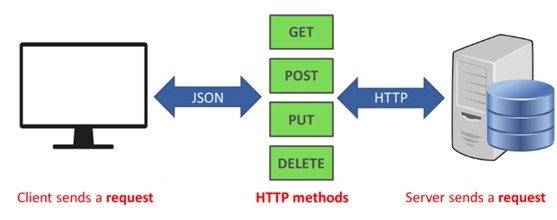
\includegraphics[scale=.6]{pic/restapi.jpg}
    \caption[ผังการทำงานของ RESTful]{ผังการทำงานของ RESTful}
    \label{fig:restapi}
  \end{center}
\end{figure}

\section{Image Processing }
เป็นกระบวนการจัดการและวิเคราะห์รูปภาพให้เป็นข้อมูลในแบบดิจิทัล โดยใช้คอมพิวเตอร์ 
เพื่อให้ได้ข้อมูลที่เราต้องการทั้งในเชิงคุณภาพและปริมาณ (ขนาด รูปร่าง) \cite{Image} โดยกระบวนการจัดการและวิเคราะห์รูปภาพที่ใช้ในโครงงานนี้ มีดังนี้

\subsection{การปรับปรุงคุณภาพของภาพ   (Image Enhancement and Restoration) }
การปรับปรุงคุณภาพของภาพเป็นการปรับปรุงหรือซ่อมแซมให้ข้อมูลภาพที่มีอยู่นั้นมี คุณภาพดีขึ้น เช่น ภาพที่ได้มาอาจมีความคมชัด (Contrast) น้อยหรือเบลอ ไม่คมชัด 
เราสามารถปรับภาพให้คมชัดได้ด้วยเทคนิค เช่น การปรับค่าความคมชัด (Contrast Enhancement) หรือการปรับเน้นเส้นขอบภาพ (Edge Enhancement) 
หรือในกรณีที่ภาพที่มี อยู่มีความไม่สมบูรณ์ เช่น มีสัญญาณรบกวน (Noise) เราสามารถใช้เทคนิคการกรองสัญญาณ ภาพ (Image Filtering) เพื่อกำจัดสัญญาณรบกวนได้

\subsection{การบีบอัดข้อมูลภาพ (Image compression)}
\begin{enumerate}
  \item \textbf{การบีบอัดแบบไม่มีการสูญเสียรายละเอียดข้อมูล (Lossless compression)} \\
  ค่าความสว่างของแต่ละจุดภาพจะยังคงอยู่เหมือนเดิมทุกประการ หรือไม่มีการเปลี่ยนแปลงค่าของแต่ละจุดภาพ 
  ซึ่งการบีบอัดวิธีนี้จะอาศัยเทคนิคการจัดเก็บข้อมูลเชิงเลขในการลดขนาดของข้อมูล
  \item \textbf{การบีบอัดแบบสูญเสียรายละเอียดข้อมูล (Lossy compression)} \\
  วิธีการนี้จะมีการเปลี่ยนแปลงค่าความสว่างของจุดภาพนั่นหมายความว่า วิธีการนี้ไม่เหมาะสมสำหรับข้อมูลภาพที่ต้องมีการจำแนกข้อมูล (Classification)
\end{enumerate}
โดยในโครงงานนี้จะใช้การใช้การบีบอัดรูปภาพแบบไม่มีการสูญเสียรายละเอียดข้อมูล (Lossless compression)
\\
\\
\\
\\
\\

\begin{figure}[!ht]
  \begin{center}
    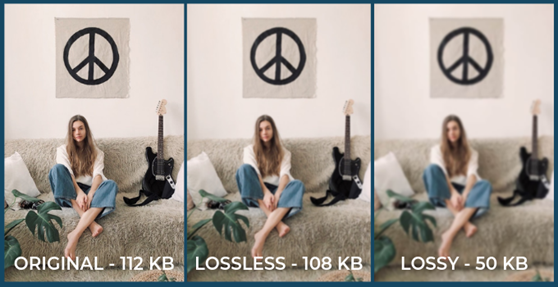
\includegraphics[scale=.7]{pic/compressiom.png}
    \caption[ความแตกต่างของการบีบอัดข้อมูล]{ความแตกต่างของการบีบอัดข้อมูล}
    \label{fig:compressiom}
  \end{center}
\end{figure}



\section{การส่งข้อมูลโดยใช้โปรโตคอลเอชทีทีพี (HyperText Transfer Protocol: HTTP) }
เป็นโปรโตคอลที่ใช้งานในด้านเว็บไซต์และในระบบอินเตอร์เน็ต สามารถสื่อสารกับข้ามแพลตฟอร์มมักจะนิยมใช้งาน HTTP 
เนื่องจากเป็นโปรโตคอลมาตรฐานที่มีมาให้ใช้งานในทุกภาษา และทุกอุปกรณ์ที่เชื่อมต่ออินเตอร์เน็ตได้ พื้นฐานของ HTTP มาจากโปรโตคอล (Transmission Control Protocol: TCP) 
ที่มีการใช้เพื่อรับ-ส่งข้อมูลในรูปแบบตามมาตรฐาน และใช้พอร์ต 80 เป็นค่าเริ่มต้น โดยผู้รับบริการ (HTTP Client) จะส่งข้อมูลผ่านคำสั่งการร้องขอแบบ POST 
เป็นคำสั่งที่ให้ส่งข้อมูลโดยแฝงข้อมูลไปกับเลขที่อยู่ไอพี (IP address) และใช้ร้องขอข้อมูลจากผู้ให้บริการ (HTTP Server) \cite{Http} ดังรูป

\begin{figure}[!ht]
  \begin{center}
    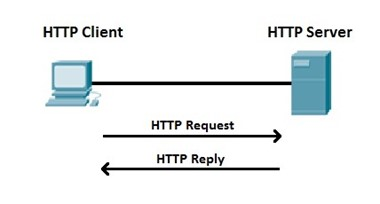
\includegraphics[scale=.8]{pic/http.jpg}
    \caption[โปรโตคอล HTTP]{โปรโตคอล HTTP}
    \label{fig:http}
  \end{center}
\end{figure}

\section{Raspberry Pi}
เครื่องคอมพิวเตอร์ขนาดเล็ก มีคุณสมบัติเด่น คือ ติดต่อ และความคุมอุปกรณ์อิเล็กทรอนิกส์ได้ โดยใน Raspberry Pi 
ได้รวมเอาซีพียู (CPU) หน่วยความจำ (Memory) และพอร์ต (Port) ซึ่งเป็นส่วนประกอบหลักสำคัญของระบบคอมพิวเตอร์เข้าไว้ด้วยกัน 
โดยทำการบรรจุเข้าไว้ในตัวถังเดียวกัน และสามารถเชื่อมต่ออินเทอร์เน็ตผ่านพอร์ตแลนหรือผ่านเครือข่ายไร้สาย \cite{PI} เช่น WiFi
	ในโครงงานนี้ได้เลือกใช้ Raspberry Pi มาเป็นอุปกรณ์ในการรับรูปภาพและค้นห้าใบหน้าในรูปภาพแบบเรียลไทม์ ส่งรูปภาพไปยังเซิร์ฟเวอร์ 
รอรับผลลัพธ์กลับมาแสดงผล ซึ่งใช้พลังงานต่ำ กินกระแสไม่เกิน 2A ในสภาวะการทำงานปกติ และสามารถเชื่อมต่ออินเทอร์เน็ตผ่านระบบไวไฟ (Wi-Fi) 
เพื่อในการรับส่งข้อมูลจากเซิร์ฟเวอร์


\section{Opensource Computer Vision (OpenCV)}
ไลบรารีโอเพ่นซอร์สที่นิยมสำหรับการประมวลผลภาพขั้นพื้นฐาน เช่น การเบลอภาพ การผสมภาพ การเพิ่มคุณภาพของภาพ 
เพิ่มคุณภาพของวิดีโอ การรู้จำวัตถุต่าง ๆ ในภาพ หรือ การตรวจจับใบหน้าหรือวัตถุต่าง ๆ ในภาพและวิดีโอได้ 
ปัจจุบัน (ปี 2022) OpenCV ได้พัฒนามาจนถึงรุ่นที่ 4 (Version 4) โดยในโครงงานนี้ได้เลือก OpenCV มาใช้ในการปรับแต่งรูป 
การตรวจจับใบหน้าแบบเรียลไทม์ และการระบุตัวตน \cite{OpenCV}

\section{Deep Learning}
ศาสตร์แขนงหนึ่งของการเรียนรู้ของเครื่อง (Machine Learning: ML) ทีเลียนแบบการทำงานของโครงข่ายประสาทของมนุษย์ (Neurons) 
โดยนำระบบโครงข่ายประสาท (Neural Network) มาซ้อนกันหลายชั้น (Layer)
และทำการเรียนรู้ข้อมูลตัวอย่าง ซึ่งข้อมูล ดังกล่าวจะถูกนำไปใช้ในการตรวจจับรูปแบบ (Pattern) หรือจัดหมวดหมู่ข้อมูล (Classify the Data)
ดังนั้นความสามารถของมันในอนาคตอาจจะเหนือมนุษย์ เนื่องจากสามารถเพิ่มพลังประมวลผลได้ไม่จำกัด 
ซึ่ง (Deep Learning: DL) คือโครงข่ายประสาทเทียม (Artificial Neural Network: ANN) ที่มีชั้นภายใน (Hidden layer) หลายชั้น 
เพื่อความสามารถในการคิดที่มากกว่าปกติ และสะท้อนสมองคนได้ดีขึ้น \cite{DEEP}
\\

\begin{figure}[!ht]
  \begin{center}
    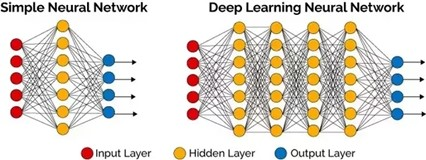
\includegraphics[scale=0.8]{pic/deep1.jpg}
    \caption[โครงสร้าง Deep Learning]{โครงสร้าง Deep Learning}
    \label{fig:deep1}
  \end{center}
\end{figure}

จะเห็นว่ามี 3 ส่วนคือ ชั้นรับข้อมูล (Input layer) ชั้นภายใน (Hidden layer) และชั้นแสดงผล (Output layer)
\begin{enumerate}
  \item ชั้นรับข้อมูล (Input layer) เป็นจุดเริ่มต้นของขั้นตอนการทำงานสำหรับ ANN จะทำหน้าที่ส่งข้อมูลไปยังแต่ละจุดต่อ (Node) ของชั้น (Layer)
  \item ชั้นภายใน (Hidden layer) เป็นส่วนที่ทำหน้าที่ส่งต่อข้อมูลไปยังชั้นแสดงผล (Output Layer) โดยแต่ละครั้งที่ข้อมูลการฝึกอบรม(Training Data) 
  ผ่านชั้น (Layer) นี้ไป แต่ละจุดต่อ (Node) จะค่อย ๆ ปรับน้ำหนัก (Weight) ให้เข้ากับข้อมูล (Data) มากขึ้นหรือถ้าอธิบายแบบเป็นทางการ 
  Hidden Layer จะคอยกักเก็บความซับซ้อนของชั้น (Layer) อื่น ๆ โดยการหาความสัมพันธ์ระหว่างคุณสมบัติ (Feature) ของข้อมูล (Data)
  \item ชั้นแสดงผล (Output layer) เป็นส่วนที่จะแสดงผล (Output) ซึ่งจำนวนจุดต่อ (Node) ในชั้นแสดงผล (Output layer) จะขึ้นอยู่กับจำนวนประเภท (Class) 
  ในข้อมูล (Data) อย่างเช่นจะสร้าง ANN เพื่อจำแนกหมากับแมว ก็ต้องมีจุดต่อแสดงผล (Output Node) 2 จุด และเมื่อใช้กับปัญหาการถดถอย (Regression Problems) ก็ต้องมี 1 จุดต่อ (Node) เท่านั้น 
  เพราะทำนาย (Predict) แค่ตัวเลข
\end{enumerate}
DL มีชั้นภายใน (Hidden layer) หลายชั้นทำให้มันสามารถคำนวณอะไรที่ซับซ้อนได้ และสามารถใช้เทคนิคต่าง ๆ ได้มากขึ้น และคิดอย่างเป็นขั้น เป็นตอนได้ดั่งรูป \\

\begin{figure}[!ht]
  \begin{center}
    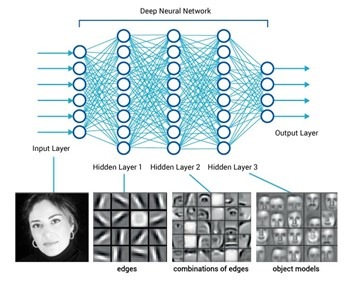
\includegraphics[scale=.9]{pic/deep2.jpg}
    \caption[Deep Learning ที่มีหลาย Hidden ayer]{Deep Learning ที่มีหลาย Hidden ayer}
    \label{fig:deep2}
  \end{center}
\end{figure}

\section{ส่วนต่อประสานกราฟิกกับผู้ใช้ (Graphical User Interface: GUI)}
การติดต่อกับผู้ใช้โดยใช้ภาพสัญลักษณ์ เป็นการออกแบบส่วนของโปรแกรมคอมพิวเตอร์ให้มีการโต้ตอบกับผู้ใช้ โดยการใช้ สัญรูป (Icon) รูปภาพ และสัญลักษณ์อื่น 
เพื่อแทนลักษณะต่าง ๆ ของโปรแกรม แทนที่ผู้ใช้จะพิมพ์คำสั่งต่าง ๆ ในการทำงาน ช่วยทำให้ผู้ใช้งานสามารถทำงานได้ง่าย และรวดเร็วขึ้น ไม่ต้องจดจำคำสั่งต่าง ๆ 
ของโปรแกรม เป็นวิธีการให้ความสะดวกแก่ผู้ใช้คอมพิวเตอร์ ให้ติดต่อสื่อสารกับระบบโดยผ่านทางภาพ เช่น ใช้เมาส์กดเลือกสัญรูป (Icon) แทนการพิมพ์คำสั่งดังแต่ก่อน 
โดยเฉพาะในบางโปรแกรมที่มีคำสั่งจำนวนมาก ซึ่งทำให้ไม่ต้องพิมพ์คำสั่งต่าง ๆ ทางแป้นพิมพ์ ช่วยทำให้เกิดความรวดเร็วในการทำงาน 
และไม่ต้องเสียเวลาในการเรียนรู้และจดจำคำสั่งที่ต้องการมากนัก เพียงดูจากไอคอนที่ปรากฏในโปรแกรมก็สามารถใช้งานได้ทันที \cite{GUI}

\section{Tkinter}
Tkinter หรือ Tk เป็นมอดูลที่พัฒนามาจาก Tk GUI Toolkit ซึ่งทางานอยู่บนระบบปฏิบัติการยูนิกซ์มาก่อนไพธอน (Python) ได้เลือกมอดูลนี้ในการพัฒนากราฟิกบนไพธอน (Python) เป็นหลัก
ประกอบไปด้วย 3 ส่วนที่สำคัญคือ วิดเจ็ต (Widgets) การจัดการรูปทรงเรขาคณิตให้กับวิดเจ็ต (Geometry management) และ การจัดการกับเหตุการณ์ต่าง ๆ (Event Handling) \cite{Tkinter} ซึ่งมีรายละเอียดดังนี้
\begin{enumerate}
  \item วิดเจ็ต (Widgets) คือ สิ่งต่าง ๆ หรือเรียกว่า อ๊อปเจ็กต์ (Object) ที่ปรากฏอยู่บนจอภาพ เช่น ปุ่ม (Button) ตัวหนังสือ (Label) เฟรม (Frame) กล่องเลือก (Checkbox) 
  วิวต้นไม้ (Tree views) แถบเลื่อน (Scrollbars) และกล่องข้อความ (Text areas) เป็นต้น
  \item การจัดการรูปทรงเรขาคณิตให้กับวิดเจ็ต (Geometry management) คือ การวางวิดเจ็ต (Widgets) ลงบนเฟรม (Frame) นั้นจะต้องกำหนดตำแหน่งในการวาง 
  โดยอาศัยศาสตร์ทางด้านเรขาคณิตเข้าช่วย เพื่อให้วิดเจ็ต (Widgets) ที่จะวางอยู่ในตำแหน่งที่เหมาะสม ซึ่งไพธอน (Python) มี 3 เมธอดในการจัดการเกี่ยวกับเรขาคณิตของวิดเจ็ต (Widgets) 
  ประกอบไปด้วยเมธอด pack(), grid() และ place()
  \item การจัดการกับเหตุการณ์ต่าง ๆ (Event Handling)  คือ เหตุการณ์ต่าง ๆ ที่ผู้ใช้งานกระทำกับวิดเจ็ต (Widgets) บน GUI เช่น การกดปุ่ม การกดปุ่มใด ๆ บนแป้นพิมพ์ 
  การเคลื่อนเมาส์ การปรับขนาดของหน้าต่างวินโดวส์ เป็นต้น เหตุการณ์ต่าง ๆ เหล่านี้จะถูกจัดการโดย Tk ซึ่งเรียกว่าวนรอบเหตุการณ์ (Event loop) โดยจะทำงานร่วมกับระบบปฏิบัติการโดยตรง 
  เช่น เมื่อเคลื่อนเมาส์ไปยังปุ่มจะส่งผลให้ปุ่มดังกล่าวจะเปลี่ยนสี และเมื่อเคลื่อนเมาส์ออกจากปุ่มจะทำให้สีของปุ่มกลับไปเป็นสีเดิม เป็นต้น
\end{enumerate}

\section{OpenFace (Open-source Face Recognition)}
มอดูลที่ใช้ในการระบุตัวตนด้วยรูปภาพใบหน้าของมนุษย์ที่ทำงานร่ามกับ DNN และเป็นมอดูลแบบโอเพนซอร์ส \cite{amos2016openface} โดยมีหลักการทำงาน ดังนี้
\begin{enumerate}
  \item ตรวจจับใบหน้าด้วยโมเดลที่ผ่านการฝึกอบรมล่วงหน้า
  \item แปลงใบหน้าสำหรับโครงข่ายประสาทเทียม ทำงานร่วมกับ OpenCV เพื่อทำให้ดวงตา และริมฝีปากล่างปรากฏในตำแหน่งเดียวกัน และสัมพันในแต่ละภาพ
  \item ใช้โครงข่ายประสาทเทียมเชิงลึก (DNN) เพื่อแสดงหรือฝังใบหน้าบนหน่วยไฮเปอร์สเฟียร์ 128 มิติ การฝังเป็นการแสดงความแตกต่างสำหรับใบหน้าของใครก็ตาม 
  ซึ่งแตกต่างจากใบหน้าอื่น ๆ การฝังนี้ทำให้เห็นคุณสมบัติที่ต่างกันมากขึ้นระหว่างใบหน้าสองใบหน้า ซึ่งทำมให้ทราบว่าใบหน้านั้นไม่น่าจะใช่คนคนเดียวกันหรือเป็นคนคนเดียวกัน 
  คุณสมบัตินี้ทำให้การจัดกลุ่ม การตรวจจับความคล้ายคลึงกัน และการจัดหมวดหมู่ทำได้ง่ายกว่าเทคนิคการจดจำใบหน้าอื่น ๆ โดยที่ระยะห่างแบบยุคลิดระหว่างคุณลักษณะต่าง ๆ 
  ไม่มีความหมาย
  \item ใช้เทคนิคการจัดกลุ่ม หรือการจัดหมวดหมู่ที่สนใจกับคุณสมบัติต่าง ๆ เพื่อทำงานการจดจำของใบหน้าบุคคล 
\end{enumerate}  


\begin{figure}[!ht]
  \begin{center}
    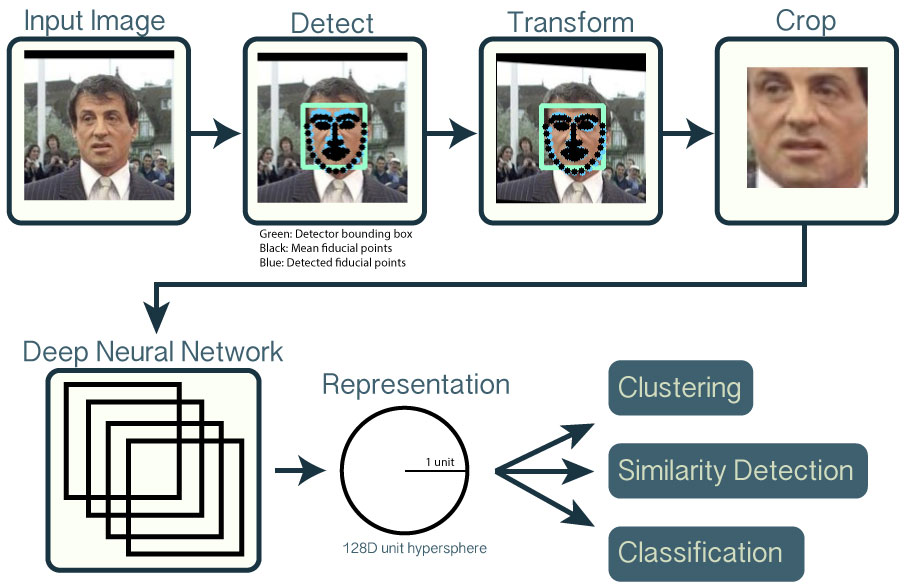
\includegraphics[scale=.25]{pic/openface.jpg}
    \caption[การทำงานของ OpenFace]{การทำงานของ OpenFace}
    \label{fig:opemface}
  \end{center}
\end{figure}



\section{\ifenglish%
\ifcpe CPE \else ISNE \fi knowledge used, applied, or integrated in this project
\else%
ความรู้ตามหลักสูตรซึ่งถูกนำมาใช้หรือบูรณาการในโครงงาน
\fi
}

\subsection{Logic and Digital Circuits และ Microprocessor and Interfacing}

ใช้ความรู้จากสองวิชานี้ในการออกแบบระบบการทำงานของอุปกรณ์ของโครงสร้างชิ้นงานใน
แต่ละส่วน และการเขียนโปรแกรมเพื่อควบคุมการทำงานของอุปกรณ์

\subsection{Digital Image Processing}

ใช้ความรู้จากวิชานี้ในการออกแบบการบีบอัดรูปภาพ การจัดเก็บรูปภาพ การทำให้รูปภาพมีคุณภาพที่ดีขึ้นเพื่อให้ความแม่นยำของการทำนายสูงขึ้น

\subsection{Deep Learning}
เรียนรู้โครงสร้าง และการทำงานของ Neuron Network เพื่อหาโมเดลการรีะบุตัวตนที่เหมาะสมกับงาน

\subsection{CPE Lab}
ใช้ในการทำ Web service และออกแบบ GUI

\section{\ifenglish%
Extracurricular knowledge used, applied, or integrated in this project
\else%
ความรู้นอกหลักสูตรซึ่งถูกนำมาใช้หรือบูรณาการในโครงงาน
\fi
}
\begin{itemize}
  \item การใช้งาน Raspbian OS ของ Raspberry Pi
  \item การตั้งค่ากล้องให้กับ Raspberry Pi และระบบ GPIO ของ Raspberry Pi เพื่อติดตั้งชุดระบายความร้อน
\end{itemize}


% \subsubsection{Subsubsection 1 heading goes here}
% Subsubsection 1 text

% \subsubsection{Subsubsection 2 heading goes here}
% Subsubsection 2 text

% \section{Third section}
% Section 3 text. The dielectric constant\index{dielectric constant}
% at the air-metal interface determines
% the resonance shift\index{resonance shift} as absorption or capture occurs
% is shown in Equation~\eqref{eq:dielectric}:

% \begin{equation}\label{eq:dielectric}
% k_1=\frac{\omega}{c({1/\varepsilon_m + 1/\varepsilon_i})^{1/2}}=k_2=\frac{\omega
% \sin(\theta)\varepsilon_\mathit{air}^{1/2}}{c}
% \end{equation}

% \noindent
% where $\omega$ is the frequency of the plasmon, $c$ is the speed of
% light, $\varepsilon_m$ is the dielectric constant of the metal,
% $\varepsilon_i$ is the dielectric constant of neighboring insulator,
% and $\varepsilon_\mathit{air}$ is the dielectric constant of air.

% \section{About using figures in your report}

% % define a command that produces some filler text, the lorem ipsum.
% \newcommand{\loremipsum}{
%   \textit{Lorem ipsum dolor sit amet, consectetur adipisicing elit, sed do
%   eiusmod tempor incididunt ut labore et dolore magna aliqua. Ut enim ad
%   minim veniam, quis nostrud exercitation ullamco laboris nisi ut
%   aliquip ex ea commodo consequat. Duis aute irure dolor in
%   reprehenderit in voluptate velit esse cillum dolore eu fugiat nulla
%   pariatur. Excepteur sint occaecat cupidatat non proident, sunt in
%   culpa qui officia deserunt mollit anim id est laborum.}\par}

% \begin{figure}
%   \centering

%   \fbox{
%      \parbox{.6\textwidth}{\loremipsum}
%   }

%   % To include an image in the figure, say myimage.pdf, you could use
%   % the following code. Look up the documentation for the package
%   % graphicx for more information.
%   % \includegraphics[width=\textwidth]{myimage}

%   \caption[Sample figure]{This figure is a sample containing \gls{lorem ipsum},
%   showing you how you can include figures and glossary in your report.
%   You can specify a shorter caption that will appear in the List of Figures.}
%   \label{fig:sample-figure}
% \end{figure}

% Using \verb.\label. and \verb.\ref. commands allows us to refer to
% figures easily. If we can refer to Figures
% \ref{fig:overview} and \ref{fig:sample-figure} by name in the {\LaTeX}
% source code, then we will not need to update the code that refers to it
% even if the placement or ordering of the figures changes.

% \loremipsum\loremipsum

% % This code demonstrates how to get a landscape table or figure. It
% % uses the package lscape to turn everything but the page number into
% % landscape orientation. Everything should be included within an
% % \afterpage{ .... } to avoid causing a page break too early.
% \afterpage{
%   \begin{landscape}
%   \begin{table}
%     \caption{Sample landscape table}
%     \label{tab:sample-table}

%     \centering

%     \begin{tabular}{c||c|c}
%         Year & A & B \\
%         \hline\hline
%         1989 & 12 & 23 \\
%         1990 & 4 & 9 \\
%         1991 & 3 & 6 \\
%     \end{tabular}
%   \end{table}
%   \end{landscape}
% }

% \loremipsum\loremipsum\loremipsum

% \section{Overfull hbox}

% When the \verb.semifinal. option is passed to the \verb.cpecmu. document class,
% any line that is longer than the line width, i.e., an overfull hbox, will be
% highlighted with a black solid rule:
% \begin{center}
% \begin{minipage}{2em}
% juxtaposition
% \end{minipage}
% \end{center}


\chapter{\ifproject%
\ifenglish Project Structure and Methodology\else โครงสร้างและขั้นตอนการทำงาน\fi
\else%
\ifenglish Project Structure\else โครงสร้างของโครงงาน\fi
\fi
}

ในบทนี้จะกล่าวถึงโครงสร้างของระบบในภาพรวม ขั้นตอนการทํางานของระบบ อุปกรณ์ หน้าที่ของอุปกรณ์ กลวิธีการต่าง ๆ และซอฟต์แวร์ที่ใช้ในระบบ โดยขั้นตอนการทํางานจะมี 9 ขั้นตอน
โดยจะแบ่งระบบออกเป็นเป็น 2 ส่วนใหญ่ ๆ คือส่วนของมอดูลกล้อง และเซิร์ฟเวอร์

\makeatletter

% \renewcommand\section{\@startsection {section}{1}{\z@}%
%                                    {13.5ex \@plus -1ex \@minus -.2ex}%
%                                    {2.3ex \@plus.2ex}%
%                                    {\normalfont\large\bfseries}}

\makeatother
%\vspace{2ex}
% \titleformat{\section}{\normalfont\bfseries}{\thesection}{1em}{}
% \titlespacing*{\section}{0pt}{10ex}{0pt}

\section{ภาพรวมโครงสร้างและการทำงานของระบบ}


\begin{figure}[ht!]
  \begin{center}
    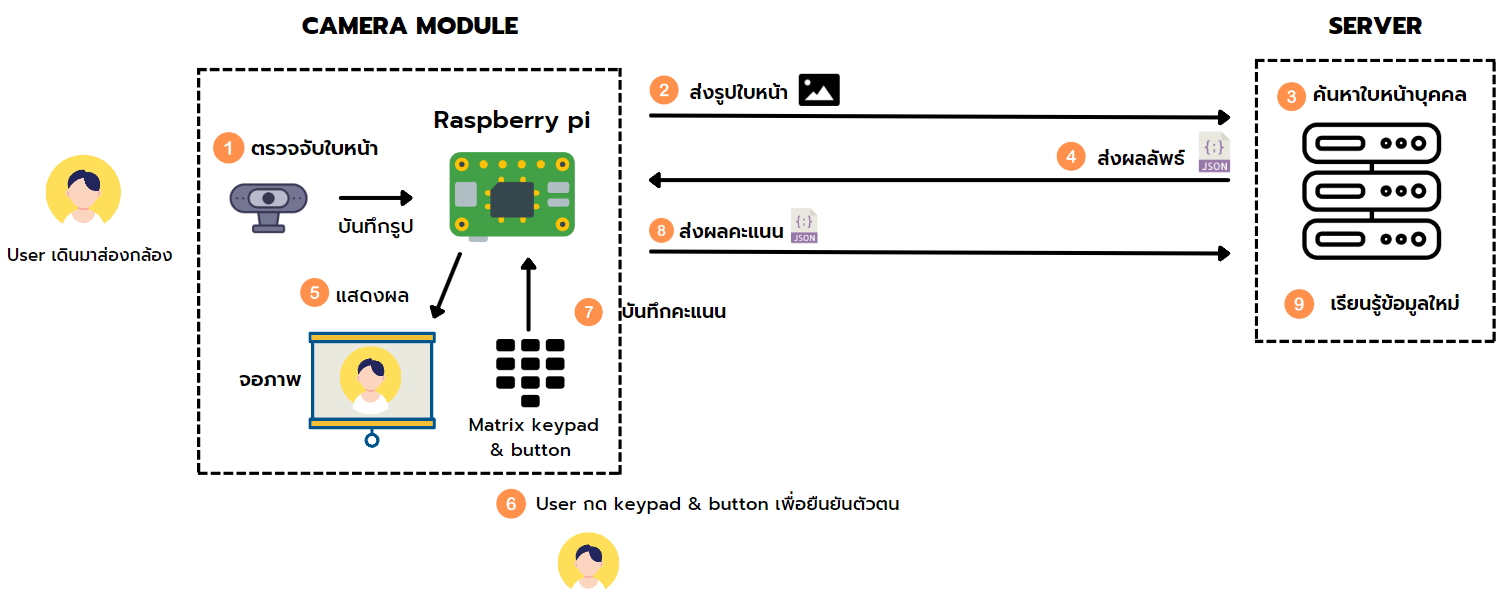
\includegraphics[scale=.5]{pic/overview.png}
  \caption[ภาพรวมของระบบ]{ภาพรวมของระบบ}
  \end{center}
  \label{fig:overview}
\end{figure}

\textbf{ขั้นตอนการทำงานของระบบมีดังนี้}
\begin{enumerate}
  \item เมื่อผู้ใช้งานเดินมาส่องกล้องแล้วมอดูลกล้องจะทำการตรวจจับใบหน้า
  \item บันทึกและส่งรูปภาพใบหน้าไปยังเซิร์ฟเวอร์ในรูปแบบแฟ้มข้อมูลภาพกราฟิกส์สีเครือข่ายใช้ได้หลายระบบ (Portable Network Graphics: PNG) 
        ผ่านโพรโทคอลเอชทีทีพี (HTTP)
  \item เชิร์ฟเวอร์รับรูปภาพแล้วบันทึกรูปภาพเพื่อนำไประบุตัวตนของรูปภาพกับแบบจำลอง (model)
  \item เชิร์ฟเวอร์ส่งผลลัพธ์ของการระบุตัวตนกลับไปยังมอดูลกล้อง (Camera module) ในรูปแบบแฟ้มข้อมูลเจซัน (JSON)
  \item แสดงผลการระบุตัวตนทางหน้าจอ
  \item ผู้ใช้งานกดแผงแป้นพิเศษ (Matrix keypad) หรือ ปุ่มกดเพื่อยืนยันตัวตน
  \item บันทึกผลการกดยืนยันตัวตน
  \item ส่งผลการยืนยันตัวตนไปยังเซิร์ฟเวอร์
  \item นำรูปภาพใบหน้าที่มีการยืนยันตัวตนไปจัดเก็นในฐานข้อมูลของบุคคนนั้น ๆ แล้วจึงทำการเรียนรู้รูปภาพใบหน้าที่ได้รับเข้ามาใหม่ในเวลากลางคืน หรือช่วงเวลาที่มีผู้ใช้งานน้อย
\end{enumerate}

\subsection{มอดูลกล้อง (Camera Module)}

\begin{figure}[ht!]
  \begin{center}
    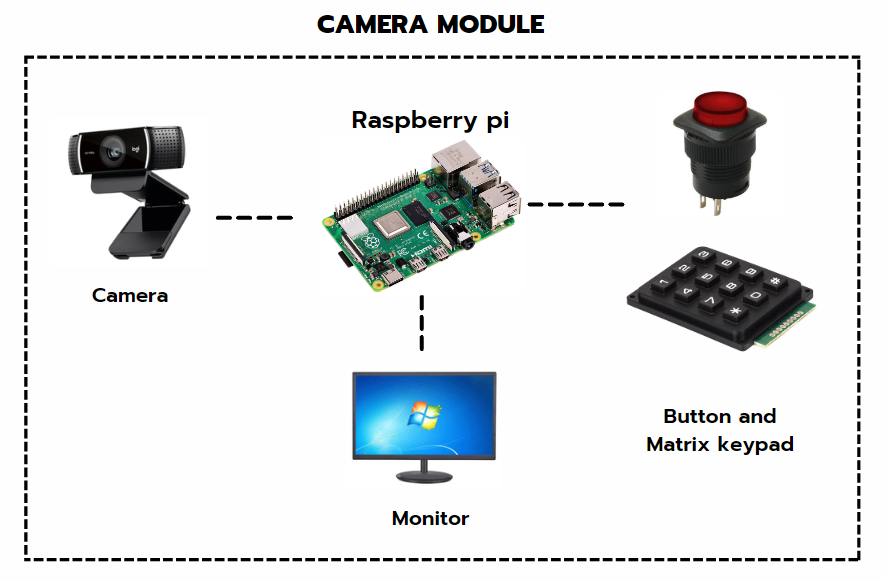
\includegraphics[scale=.45]{pic/camera_module.png}
    \caption[ส่วนประกอบต่าง ๆ ที่ใช้ในมอดูลกล้อง (Camera Module)]{ส่วนประกอบต่าง ๆ ที่ใช้ในมอดูลกล้อง (Camera Module)}
    \label{fig:camera}
  \end{center}
\end{figure}

\textbf{อุปกรณ์ที่ใช่ในมอดูลกล้องสำหรับการตรวจจับใบหน้ามีดังนี้}
\begin{enumerate}
  \item Raspberry Pi 4 Model B : แพลตฟอร์มที่ใช้ในการค้นหาใบหน้าบุคคล ซึ่งคุณสมบัติที่จำเป็นได้แก่ 
  มีขนาดเล็ก สามารถส่งข้อมูลผ่านเครื่องข่ายไร้สายไวไฟ (WI-FI) หรือผ่านเครือข่ายที่ใช้สาย (LAN) สามารถอ่านข้อมูลภาพจากกล้องถ่ายภาพ 
  และส่งรูปภาพไปยังเซิร์ฟเวอร์และรอรับผลลัพธ์ และส่งผลลัพธ์จากปุ่มกลับไปยังเซิร์ฟเวอร์
  \item Camera : กล้องเว็บแคมที่มีใช้มาการส่งภาพใบหน้าไปยัง Raspberry Pi
  \item Monitor : หน้าจอแสดงผลที่ใช้ในการแสดงผลลัพธ์ของการระบุตันตน
  \item Button และ Matrix keypad : ใช้ในการรับการให้คะแนนการแสดงผลลัพธ์และแก้ไขความถูกผิดของการแสดงผลลัพธ์
\end{enumerate}

\subsection{การส่งข้อมูลไปยังเซิร์ฟเวอร์}
การส่งรูปภาพจากมอดูลกล้องไปยังเซิร์ฟเวอร์นั้นในมอดูลกล้องใช้คำสั่ง ภาษาไพธอน (Python) ในการใช้สั่งคำส่งของระบบ (System)
คือเคิร์ล  (Client for URLs: cURL) ในการส่งรูปภาพผ่าน HTTP ไปยังเซิร์ฟเวอร์ที่เป็น (RESTful Web Services: RWS)
ผ่านเลขที่อยู่ไอพี (IP Address) ของเซิร์ฟเวอร์ โดย RWS นั้นใช้ Flask Framework 
ในการสร้างเนื่องจาก Flask Framework นั้นใช้ภาษาไพธอน (Python) ในการเขียนทำให้มีความสะดวกในการเรียก OpenCV มาใช้งาน

\subsection{การแสดงผลการระบุตัวตน}
การแสดงผลที่หน้าจอที่เชื่อมต่อกับ Raspberry Pi โดยรับข้อมูลมาจากเซิร์ฟเวอร์ที่ส่งข้อมูลบุคคลที่มีความใกล้เคียงจำนวน 5 คน 
แต่จะต้องมีความใกล้เคียงกับรายชื่อในฐานข้อมูลมากกว่า 80 เปอร์เซ็นต์จึงจะส่งผลลัพธ์ได้ แต่ถ้าไม่มีความใกล้เคียงมากกว่า 80 เปอร์เซ็นต์ก็จะแสดงผลว่า ``ไม่รู้จัก"
โดยเซิร์ฟเวอร์ส่งข้อมูลแบบ JSON กลับมาให้ Raspberry Pi แบบการสนอง (Response) เมื่อรับข้อมูลจากเซิร์ฟเวอร์จะทำการนำไปแสดงผลที่หน้าจอ 
และเมื่อผู้ใช้งานยืนยันตัวตนแล้วนั้นจะส่งผลการยืนยันตัวตนกลับไปยังเซิร์ฟเวอร์เพื่อทำการย้ายรูปภาพใบหน้าไปยังที่จัดเก็บตามรายชื่อในฐานข้อมูล

\begin{figure}[!ht]
  \begin{center}
    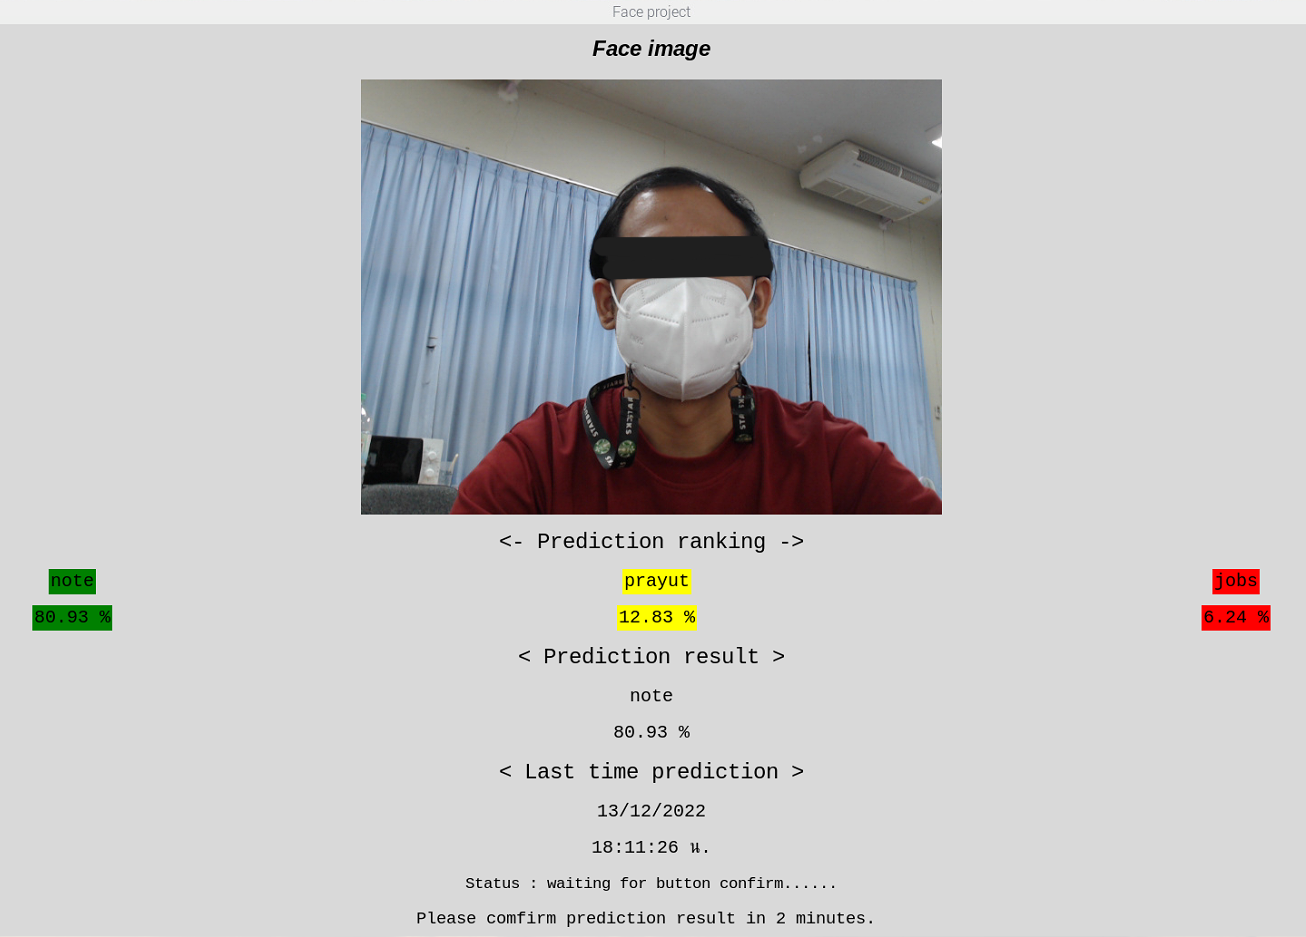
\includegraphics[scale=.45]{pic/result_page_blind.png}
  \caption[แสดงผลลัพธ์การระบุตัวตน]{แสดงผลลัพธ์การระบุตัวตน}
  \end{center}
  \label{fig:predict_result}
\end{figure}


\subsection{เซิร์ฟเวอร์ (Server)}
ทำหน้าที่ในการเป็นเว็ปเซอร์วิส (Web service) ในการรับรูปภาพเพื่อนำรูปภาพมาระบุตัวตนโดยใช้ OpenCV
เพื่อบอกว่ารูปภาพใบหน้าที่ได้รับเข้ามามีความใกล้เคียงกับบุคคลในฐานข้อมูล โดยแบบจำลอง (model) ที่ใช้ในการระบุตัวตนนั้นมาจาก OpenFace ที่ได้เรียนรู้รูปภาพใบหน้าจากที่จัดเก็บ (Storage) 
จนได้แบบจำลอง (model) ไปใช้งานในการระบุตัวตน และเมื่อ OpenCV บอกผลลัพธ์ได้แล้วจึงทำการส่งการตอบสนอง (Response) 
กลับไปยังมอดูลกล้อง แล้วทำการรอรับข้อมูลการยืนยันตัวตนเพื่อนำรูปภาพที่ได้รับเข้ามาใหม่นั้นย้ายไปยังตำแหน่งที่จัดเก็บของบุลคลนั้น ๆ ในเวลากลางคืนหรือเสลาที่มีผู้ใช้งานน้อยของทุก 
วัน เซิร์ฟเวอร์จะทำการสั่ง OpenFace เรียนรู้รูปภาพใหม่ และนำแบบจำลอง (model) ใหม่ไปใช้งาน โดยเซิร์ฟเวอร์จะมีความต้องการด้านฮาร์ดแวร์คือต้องมีความจุมากกว่า 1 เทราไบต์  (Terabyte) 
หน่วยความจำขนาด 16 จิกะไบต์ (Gigabyte) ในการประมวลผล

\subsection{การระบุตัวตน}
การระบุตัวตนจะใช้ภาพถ่ายใบหน้าที่ได้รับมาจากมอดูลกล้องใช้ OpenFace ในการระบุตัวตนโดยรับตัวแบบจำลอง (model) ที่ใช้ในการทำนายรูปภาพใบหน้าว่ามีความใกล้เคียงมากกับบุคคลในฐานข้อมูล
แล้วทำการคัดกรองรูปภาพที่มีความใกล้เคียงกับฐานข้อมูลมากกว่า 80 เปอร์เซ็นต์ จึงจะส่งข้อมูลไปให้เซิร์ฟเวอร์ทำการส่งผลลัพธ์การระบุตัวตนกลับไปยังมอดูลกล้อง
แต่เมื่อไม่มีรูปภาพใบหน้าที่มีความใกล้เคียงกับฐานข้อมูลมากกว่า 80 เปอร์เซ็นต์จะส่งไปบอกเซิร์ฟเวอร์ เพื่อให้เซิร์ฟเวอร์ทำการส่งผลลัพธ์กลับไปยังมอดูลกล้องว่า ``ไม่รู้จัก"

\subsection{การจัดเก็บรูปภาพใบหน้า}
จัดเก็บรูปภาพใบหน้าลงในที่เก็บข้อมูลในเครื่อง (Local storage) บนเซิร์ฟเวอร์โดยแบ่งเป็นแฟ้มข้อมูล \\(Folder) 
ในแต่ละแฟ้มก็จะเป็นรายชื่อของบุคคลที่ลงทะเบียนหรือเป็นผู้ที่ใช้งานห้อง 
โดยเมื่อได้รับรหัสการยืนยันตัวตนในกรณีที่ความแม่นยำการระบุตัวตนน้อยกว่า 80 เปอร์เซ็นต์จากการระบุตัวตนจะทำการเที่ยบรหัสที่ได้รับเข้ามากับรหัสที่จัดเก็นบนฐานข้อมูล 
เมื่อผลลัพธ์การเทียบมีความถูกต้องจะย้ายรูปภาพไปยังแฟ้มของบุคคลนั้น แต่ถ้าผลลัพธ์การเทียบไม่ถูกต้อง
จะย้ายรูปภาพไปยังแฟ้มของอื่น ๆ เพื่อให้ผู้ดูแลมาทำการเทียบด้วยตัวอง

\begin{figure}[ht]
  \begin{center}
    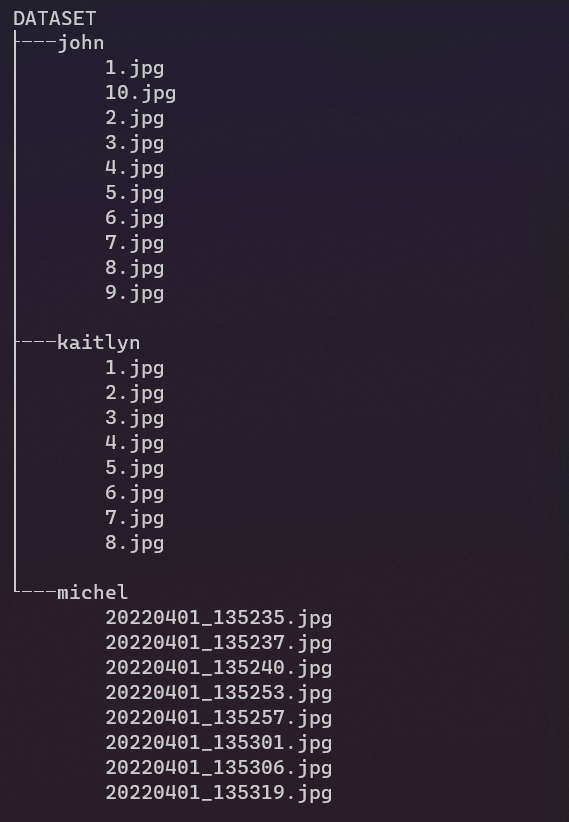
\includegraphics[scale=.5]{pic/dataset.png}
  \caption[แผนภาพแสดงการจัดเก็บรูปภาพใบหน้า]{แผนภาพแสดงการจัดเก็บรูปภาพใบหน้า}
  \end{center}
  \label{fig:folder}
\end{figure}


\subsection{การเรียนรู้รูปภาพ}
ใช้ OpenFace ในการเรียนรู้รูปภาพ โดย OpenFace นั้นใช้ภาษาไพธอน (Python) ในการเขียนโปรแกรมเพื่อเรียนรู้รูปภาพใบหน้า เริ่มจากการนำรูปภาพของบุคคลที่บันทึกไว้ในที่จัดเก็บ (Storage) 
และรายชื่อของบุคคลที่มีรูปภาพใบหน้าในที่จัดเก็บ (Storage) แล้วทำการเรียนรู้ด้วย OpenFace จะได้แบบจำลองการเรียนรู้เพื่อนำไปใช้ในการระบุตัวตนของบุคคล 
โดยขั้นตอนการเรียรรู้จะใช้เวลาขึ้นอยู่กับจำนวนของรูปภาพที่จัดเก็บไว้และใช้ทรัพยากรในการเรียนรู้รูปภาพใบหน้าที่สูงจึงนำ OpenFace ไปทำการเรียนรู้ที่เซิร์ฟเวอร์

% do with it:---it was the black kitten's fault entirely~\cite{aiw}.  For the

\chapter{\ifproject%
\ifenglish Experimentation and Results\else การทดลองและผลลัพธ์\fi
\else%
\ifenglish System Evaluation\else การประเมินระบบ\fi
\fi}

% ในบทนี้จะทดสอบเกี่ยวกับการทำงานในฟังก์ชันหลักๆ
ในบทนี้จะทดสอบระบบการยืนยันตัวตนด้วยการใช้ภาพใบหน้า โดยมีผู้ทดลอง 5 คน 
ทำการทดลองเป็นเวลา 5 วันเพื่อดูผลการทดลองในแต่ละวัน ได้แก่ ความแม่นยำของการระบุตัวตนด้วยใบหน้า 
เวลาในการตรวจจับใบหน้าตลอดถึงการแสดงผล และความพึงพอใจของผู้ทดลองต่อระบบ

\section{ความแม่นยำของการตรวจจับใบหน้า}
การทดสอบนี้จะเป็นการทดสอบเพื่อวัดผลความแม่นยำในการตรวจจับภาพใบหน้า

\begin{figure}[!ht]
  \begin{center}
    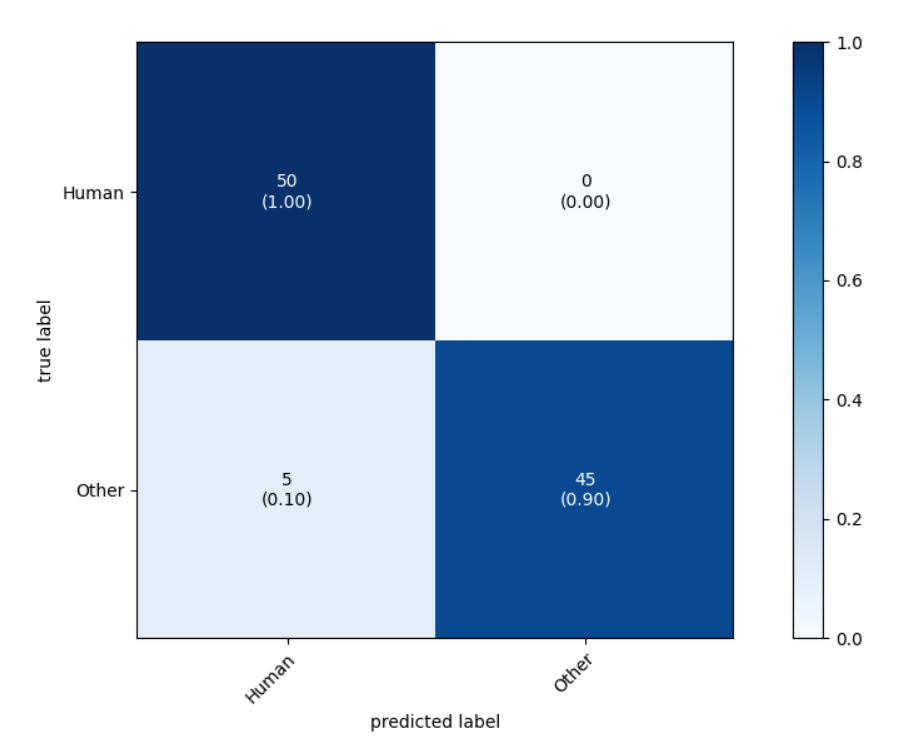
\includegraphics[scale=.45]{pic/face_result.png}
    \caption[กราฟแสดงความแม่นยำของการตรวจจับใบหน้า]{กราฟแสดงความแม่นยำของการตรวจจับใบหน้า}
    \label{fig:acc_graph}
  \end{center}
\end{figure}

\indent จากกราฟจะสามารถคำนวนความแม่นยำได้ดังสูตร 

\section{ความแม่นยำของการระบุตัวตนด้วยใบหน้าในแต่ละวัน}
การทดสอบนี้จะเป็นการทดสอบเพื่อวัดผลความแม่นยำในการระบุตัวตนนั้นมีความแม่นยำเพิ่มขึ้นหรือลดลงตามวันเวลาที่ตรวจจับภาพใบหน้า
โดยจะบันทึกความแม่นยำหลังจากการทำนายผลรูปภาพใบหน้าทุก ๆ ครั้งที่มีการตรวจจับภาพใบหน้าและนำไปแสดงผล

\begin{figure}[!ht]
    \begin{center}
      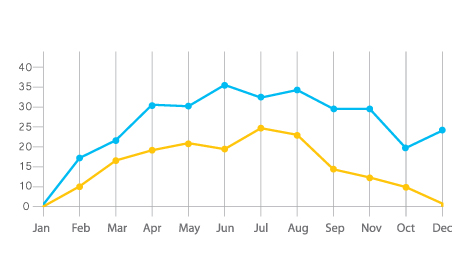
\includegraphics[scale=.6]{pic/graph_acc.jpg}
      \caption[กราฟแสดงความแม่นยำของการระบุตัวตนในแต่ละวัน]{กราฟแสดงความแม่นยำของการระบุตัวตนในแต่ละวัน}
      \label{fig:face_graph}
    \end{center}
  \end{figure}

\indent จากกราฟจะเห็นได้ว่าความแม่นยำเมื่อเวลาในการจัดเก็บข้อมูลนั้นมากขึ้นก็จะทำให้ความแม่นยำสูงขึ้น แต่จะมีจุดที่ความแม่นยำสูงที่สุดและลดลงเรื่อยเนื่องจาก
ข้อมูลรูปภาพใบหน้ามีจำนวนที่เกินไปทำให้ความแม่นยำนั้นจะไม่สูงไปกว่าจัดนี้อีกแล้ว

\section{เวลาในการประมวลผลรูปภาพใบหน้า}
การทดสอบต่อไปนี้เป็นการทดสอบเพื่อวัดผลว่าเวลาในการประมวลผลรูปภาพใบหน้าตลอดจนระบุตัวตนที่ออกแบบนั้น
มีเวลาาที่มากหรือน้อยเพียงใดจากการบันทึกผลที่ Raspberry Pi โดยจะเปรียบเทียบที่วัดได้ในครั้งที่มีการตรวจจับภาพใบหน้า
เปรียบเทียบออกมาเป็นกราฟเส้นดังนี้
  
\begin{figure}[!ht]
  \begin{center}
    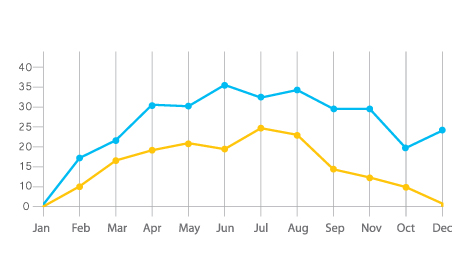
\includegraphics[scale=.7]{pic/graph_acc.jpg}
    \caption[กราฟแสดงเวลาในการประมวลผลของระบบในแต่ละวัน]{กราฟแสดงเวลาในการประมวลผลของระบบในแต่ละวัน}
    \label{fig:time_graph}
  \end{center}
\end{figure}
\newpage
\indent จากกราฟจะเห็นได้ว่าเวลาในการประมวลผลรูปภาพใบหน้า ส่งรูปภาพไปยังเซิร์ฟเวอร์ การระบุตัวตน และการส่งผลลัพธ์กลับมาแสดงผลในหน้าจอนั้นมีเวลาเฉลี่ย .... มิลลิวินาที



\section{ความพึงพอใจของการทดลอง}
จากการทดลองที่ห้องวิจัย OASYS ได้ทำการบันทึกผลความพึงพอใจของผู้ทดลองต่อระบบระบุตัวตนด้วยรูปภาพใบหน้าบุคคลที่ โดยจะได้ผลสรุปดังนี้

\begin{figure}[!ht]
    \begin{center}
      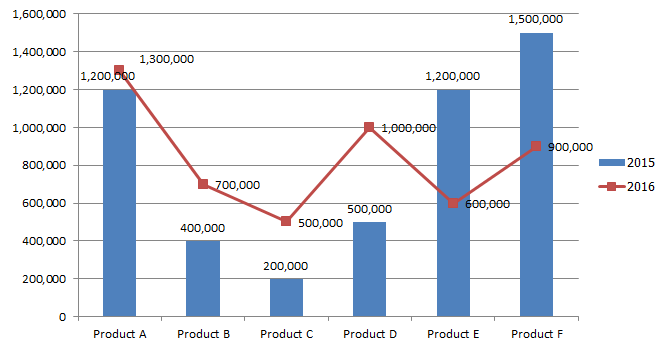
\includegraphics[scale=.5]{pic/bar_graph.png}
      \caption[กราฟแสดงความพึงพอใจของผู้ทดลอง]{กราฟแสดงความพึงพอใจของผู้ทดลอง}
      \label{fig:bar_graph}
    \end{center}
  \end{figure}
\ifproject
\chapter{\ifenglish Conclusions and Discussions\else บทสรุปและข้อเสนอแนะ\fi}

\section{\ifenglish Conclusions\else สรุปผล\fi}

ในการทำโครงงานระบบการยืนยันตัวตนด้วยการใช้ภาพใบหน้าเพื่อเข้าสู่สถานที่ด้วยการใช้กลวิธีการเรียนรู้ของเครื่องแบบต่อเนื่องสามารถพัตนาให้มอดูลตรวจจับใบหน้านั้นตรวจจับใบหน้าได้แม่นยำถึง 100 เปอร์เซ็นต์ 
เมื่อนำไปติดตั้งทดสอบสามารถทำงานได้อย่างถูกต้อง ใช้พื้นที่ติดตั้งน้อย และเวลาเฉลี่ยในการทำงานระหว่างเซิร์ฟเวอร์กับมอดูลกล้องคือ 455.618 มิลลิวินาที


\section{\ifenglish Challenges\else ปัญหาที่พบและแนวทางการแก้ไข\fi}

ในการทำโครงงานนี้ พบว่าเกิดปัญหาหลัก ๆ ดังนี้
\begin{enumerate}
    \item เมื่อรูปภาพใบหน้ามีความคมชัดน้อย จะทำให้แบบจำลองการตรวจจับใบหน้าไม่สามารถนำรูปภาพใบหน้าไปเรียนรู้รูปภาพใบหน้าเป็นแบบจำลองการรระบุตัวตน จึงต้องมีการใช้การปรับรูปภาพให้ดีขึ้น เช่น การลดสัญญาณรบกวนที่เกิดขึ้นในภาพ การเพิ่มความคมชัด 
    และการบีบอัดคงสัญญาณ เป็นต้น
    \item ในการตรวจจับรูปภาพใบหน้าบนมอดูลกล้อง เมื่อผู้ใช้งานขยับตัวในขณะที่กล้องกำลังโฟกัสใบหน้าบุคคล จะทำให้รูปภาพใบหน้าบุคคลไม่ชัดส่งผลให้ผลลัพธ์ของรูปภาพที่ส่งไประบุตัวตนมีความผิดพลาดสูง 
    จึงมีการกำหนดข้อตกลงให้ผู้ใช้อยู่นิ่งในตอนที่กล้องกำลังโฟกัส
    \item เมื่อมอดูลกล้องเปิดใช้งานเป็นเวลานานจะเกิดปัญหาหน่วยความจำชั่วคราวเต็ม ซึ่งจะต้องทำการเปิดโปรแกรมใหม่
    \item เมื่ออินเทอร์เน็ตมีปัญหา เช่น หลุด หรือ ไฟดับ จะทำให้โปรแกรมบนมอดูลกล้องนั้นค้างต้องมีการตรวจสอบอินเทอร์เน็ตทุกวัน
    \item การจ่ายไฟให้กับมอดูลกล้องจะต้องใช้ตัวปรับกระแสไฟที่มีกำลังการจ่ายไฟที่เพียงพอ เนื่องจากกำลังไฟที่น้อยไปจะทำให้ประสิทธิภาพของ Raspberry Pi ลดลง
    \item ในขั้นตอนการกดปุ่มกดตัวเลขเพื่อยืนยันตัวตน เมื่อผู้ใช้กดปุ่มค้างจะทำให้เลขยืนยันตัวตนจะผิดพลาดไปด้วย และเมื่อหน่วงเวลาของปุ่มกดมากไปจะทำให้ผู้ใช้กรอกรหัสการยืนยันตัวตนผิดพลาด
\end{enumerate}



\section{\ifenglish%
Suggestions and further improvements
\else%
ข้อเสนอแนะและแนวทางการพัฒนาต่อ
\fi
}

ข้อเสนอแนะเพื่อพัฒนาโครงงานนี้ต่อไป มีดังนี้
\begin{enumerate}
    \item สามารถที่จะพัฒนาแบบจำลองการเรียนรู้รูปภาพใบหน้า โดยใช้กลวิธีการเรียนรู้ของเครื่องในรูปแบบอื่น ๆ เพื่อเพิ่มความแม่นยำในการระบุตัวตนขณะที่ใส่หน้ากากอนามัยสูงขึ้น
    \item ในการออกแบบมอดูลกล้องสามารถออกแบบให้กล่องเก็บ Raspberry Pi นั้นมีขนาดเล็กลงก็จะใช้พื้นที่ลดลงได้
    \item ปุ่มกดยืนยันตัวตนสามารถที่จะเปลี่ยนไปใช้ปุ่มที่ใช้ระบบอินฟราเรด หรือ ระบบยืนยันแบบการชูจำนวนนิ้วเพื่อบ่งบอกตัวเลขผ่านกล้อง (Hand Gesture Recognition) ก็จะลดการสัมผัสทำให้ลดการแพร่กระจายของโรคติดต่อ 
    \item ควรพัฒนาแบบจำลองการตราจจับใบหน้าให้มีประสิทธิภาพมากขึ้น เนื่องจากเมื่อประสิทธิภาพมากขึ้นจะทำให้การตรวจจับใบหน้านั้นรวดเร็วยิ่งขึ้น
    \item ควรพัฒนาวิธีการเพิ่มความชัดของรูปภาพใบหน้า เนื่องจากมีผลต่อความแม่นยำในการระบุตัวตน
    \item ควรสำรวจพื้นที่ติดตั้งมอดูลกล้อง เนื่องจากต้องพิจารณาสภาพแสงของพื้นที่ติดตั้งเพื่อพัฒนาการปรับแต่งรูปภาพให้สว่าง หรือ มืด ซึ่งมีผลต่อความแม่นยำในการระบุตัวตน
    \item สามารถใช้กล้องแบบโฟกัสคงที่ เพื่อกำหนดระยะของการตรวจจับใบหน้าที่ชัดเจน ทำให้สามารถลดการความพร่ามัวของรูปภาพใบหน้าส่งผลให้ความแม่นยำในการระบุตัวตนสูงขึ้น 
\end{enumerate}

\fi

\bibliography{myReport}

\ifproject
\normalspacing
\appendix
\chapter{อุปกรณ์ต้นแบบและการแสดงผลบนหน้าจอ}



\section{รูปอุปกรณ์ที่ใช้ในการตรวจจับภาพใบหน้าและรับคำสั่งยืนยัน}

\begin{figure}[!ht]
  \begin{center}
    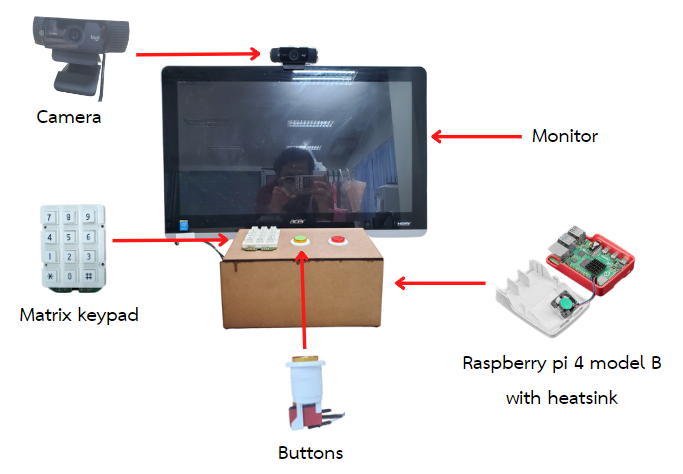
\includegraphics[scale=.6]{pic/overall_module.png}
    \caption[อุปกรณ์ตรวจจับใบหน้า แสดงผลและรับผล]{อุปกรณ์ตรวจจับใบหน้า แสดงผลและรับผล}
    \label{fig:module_pi}
  \end{center}
\end{figure}



% Text for a section in the first appendix goes here.

% test ทดสอบฟอนต์ serif ภาษาไทย
\begin{figure}[!ht]
  \begin{center}
    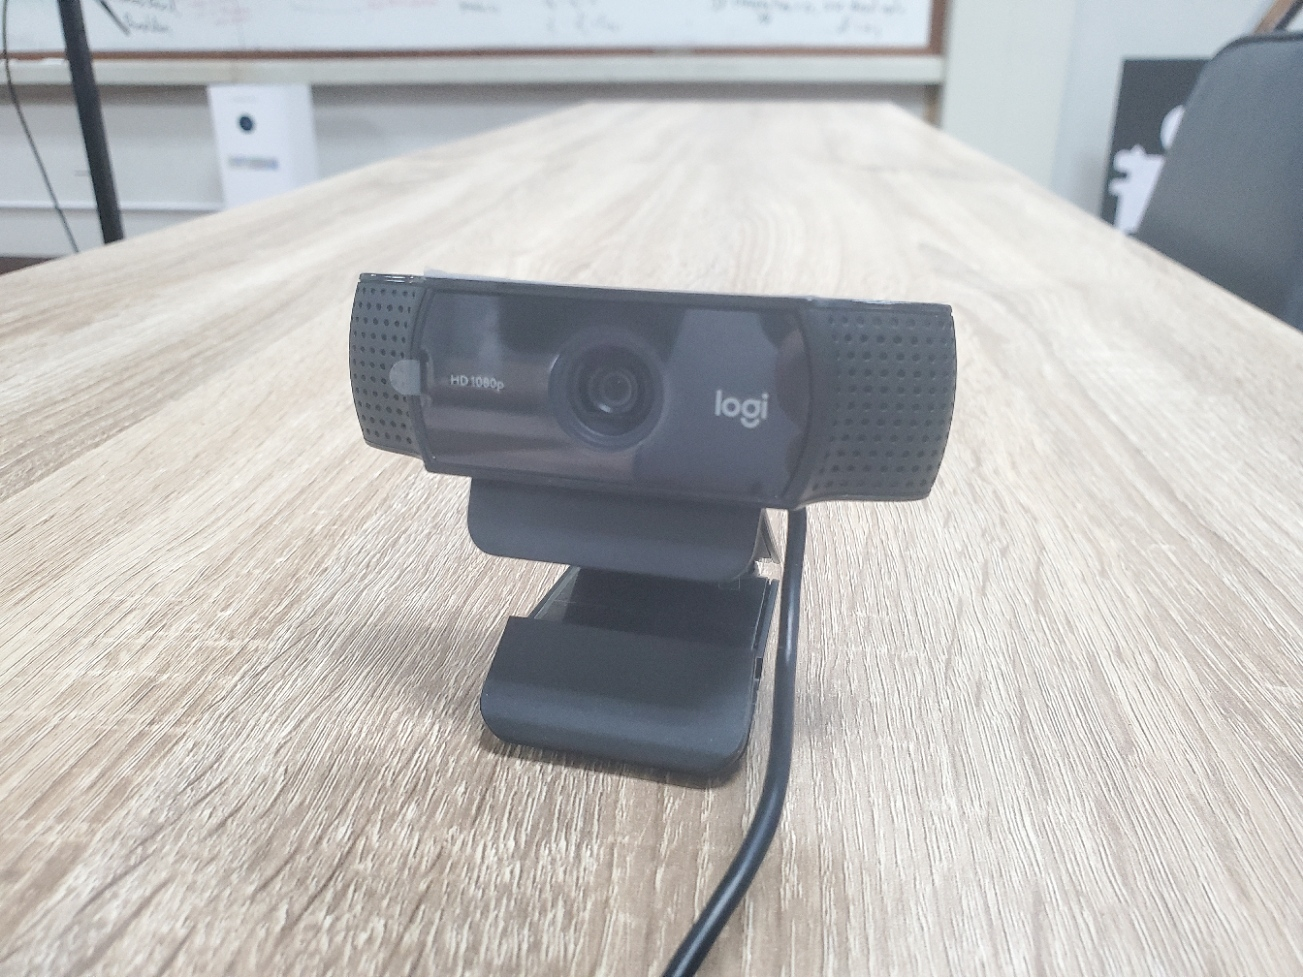
\includegraphics[scale=.15]{pic/camera.jpg}
    \caption[กล้องที่ใช้ในการตรวจจับใบหน้าบุคคล]{กล้องที่ใช้ในการตรวจจับใบหน้าบุคคล}
    \label{fig:camera_logi}
  \end{center}
\end{figure}

% \begin{figure}[!ht]
%   \begin{center}
%     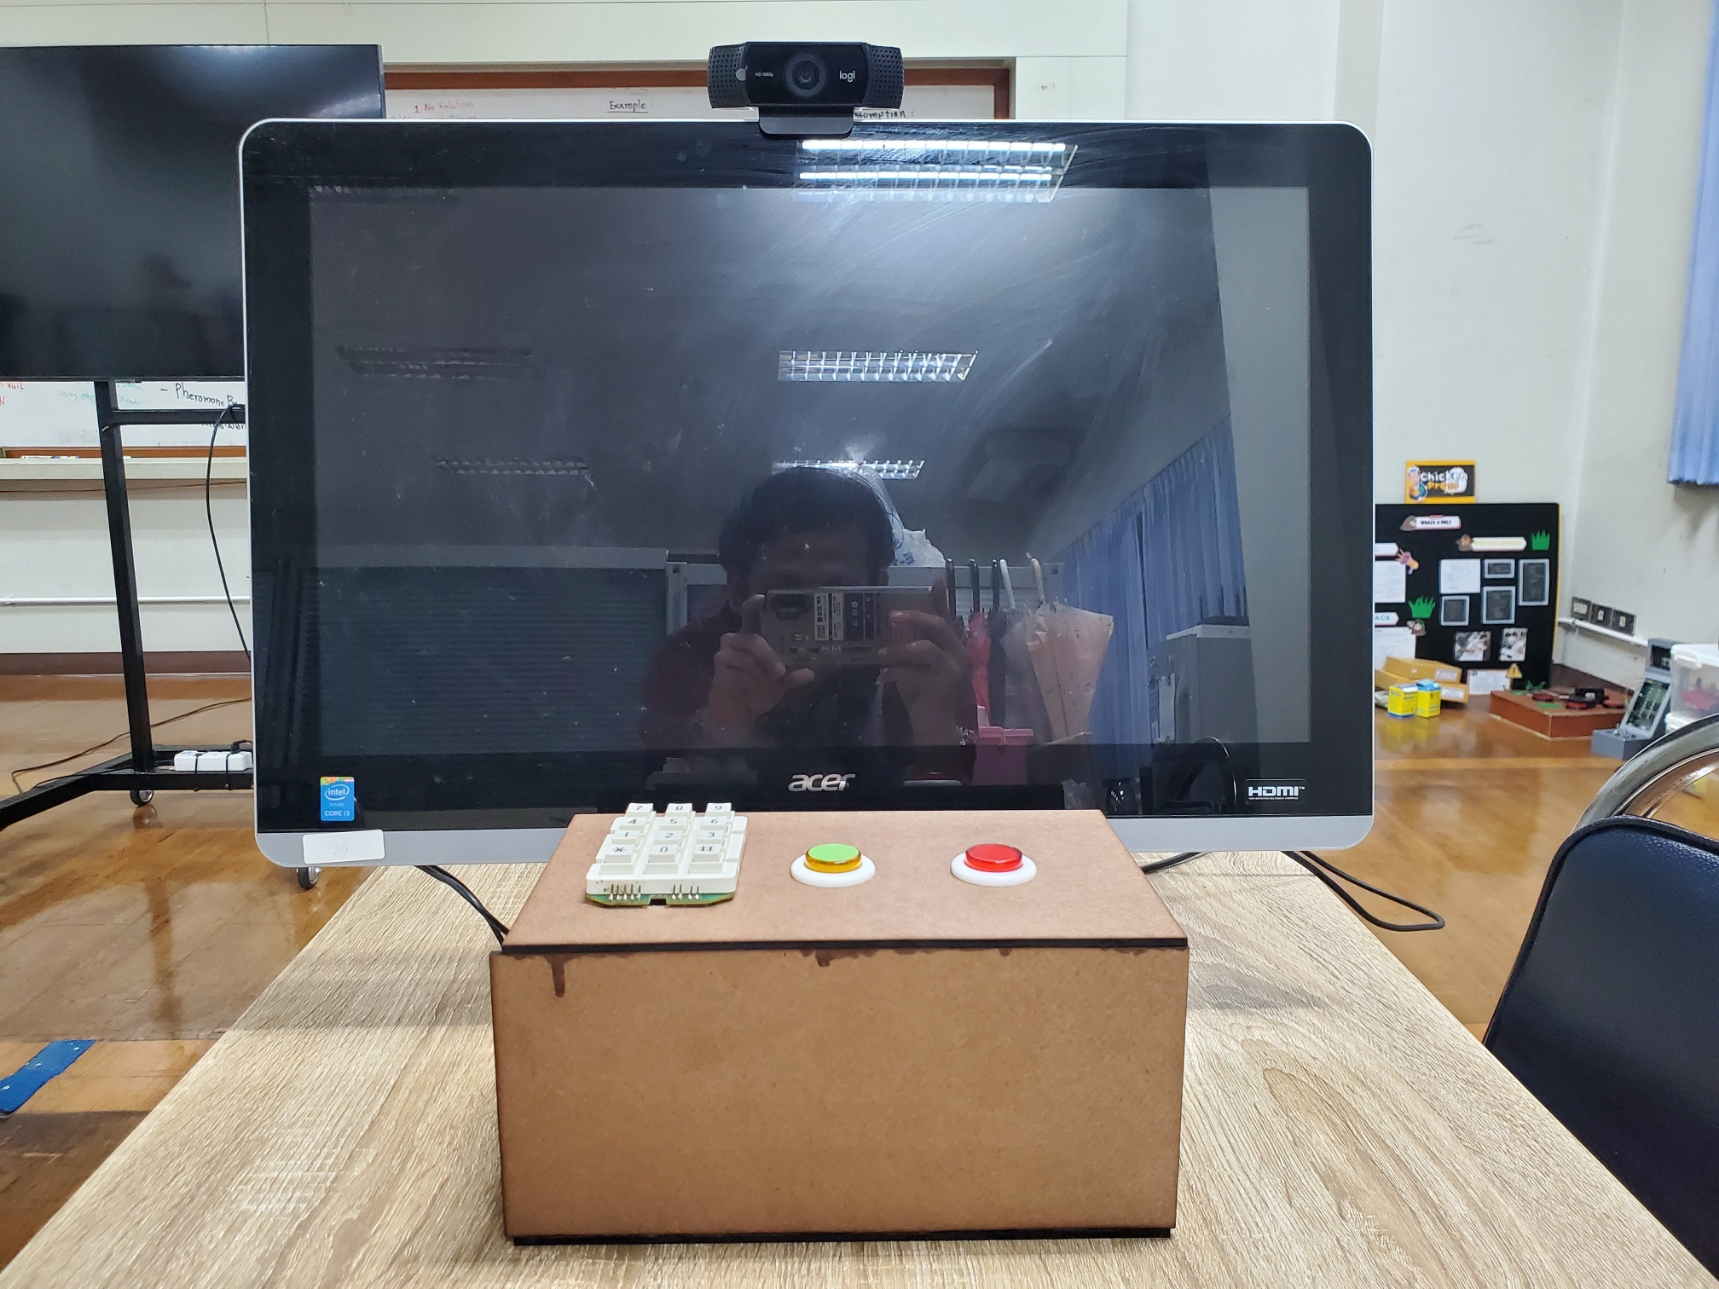
\includegraphics[scale=.1]{pic/system.jpg}
%     \caption[face detection module]{มอดูลที่ใช้ในการระบุตัวตนด้วยรูปภาพใบหน้าและแสดงผล}
%     \label{fig:face_module}
%   \end{center}
% \end{figure}

\begin{figure}[!ht]
  \begin{center}
    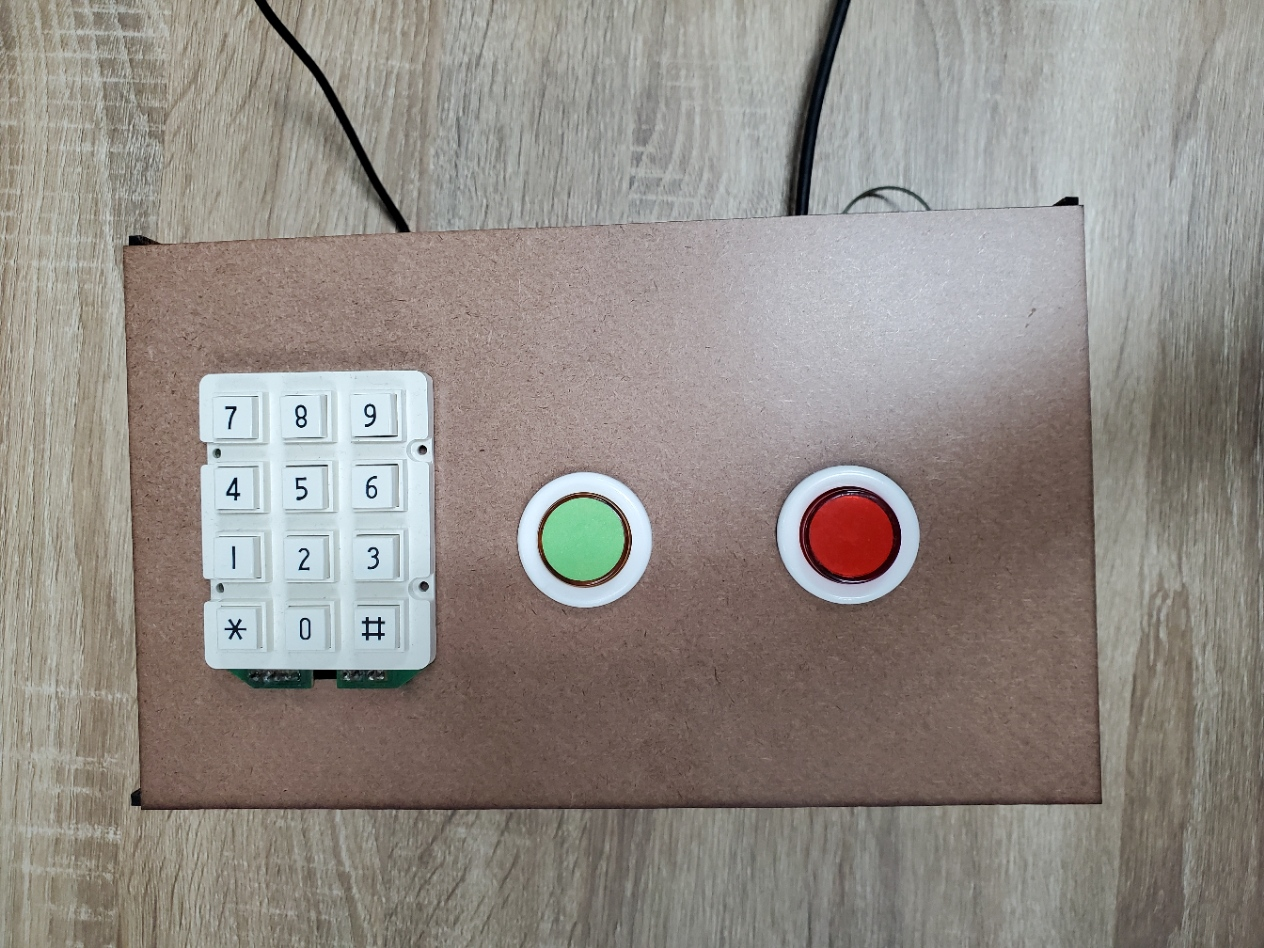
\includegraphics[scale=.17]{pic/rpi_top.jpg}
    \caption[ปุ่มกดยืนยันความถูกต้องของการระบุตัวตน]{ปุ่มกดยืนยันความถูกต้องของการระบุตัวตน}
    \label{fig:button_module}
  \end{center}
\end{figure}

\begin{figure}[!ht]
  \begin{center}
    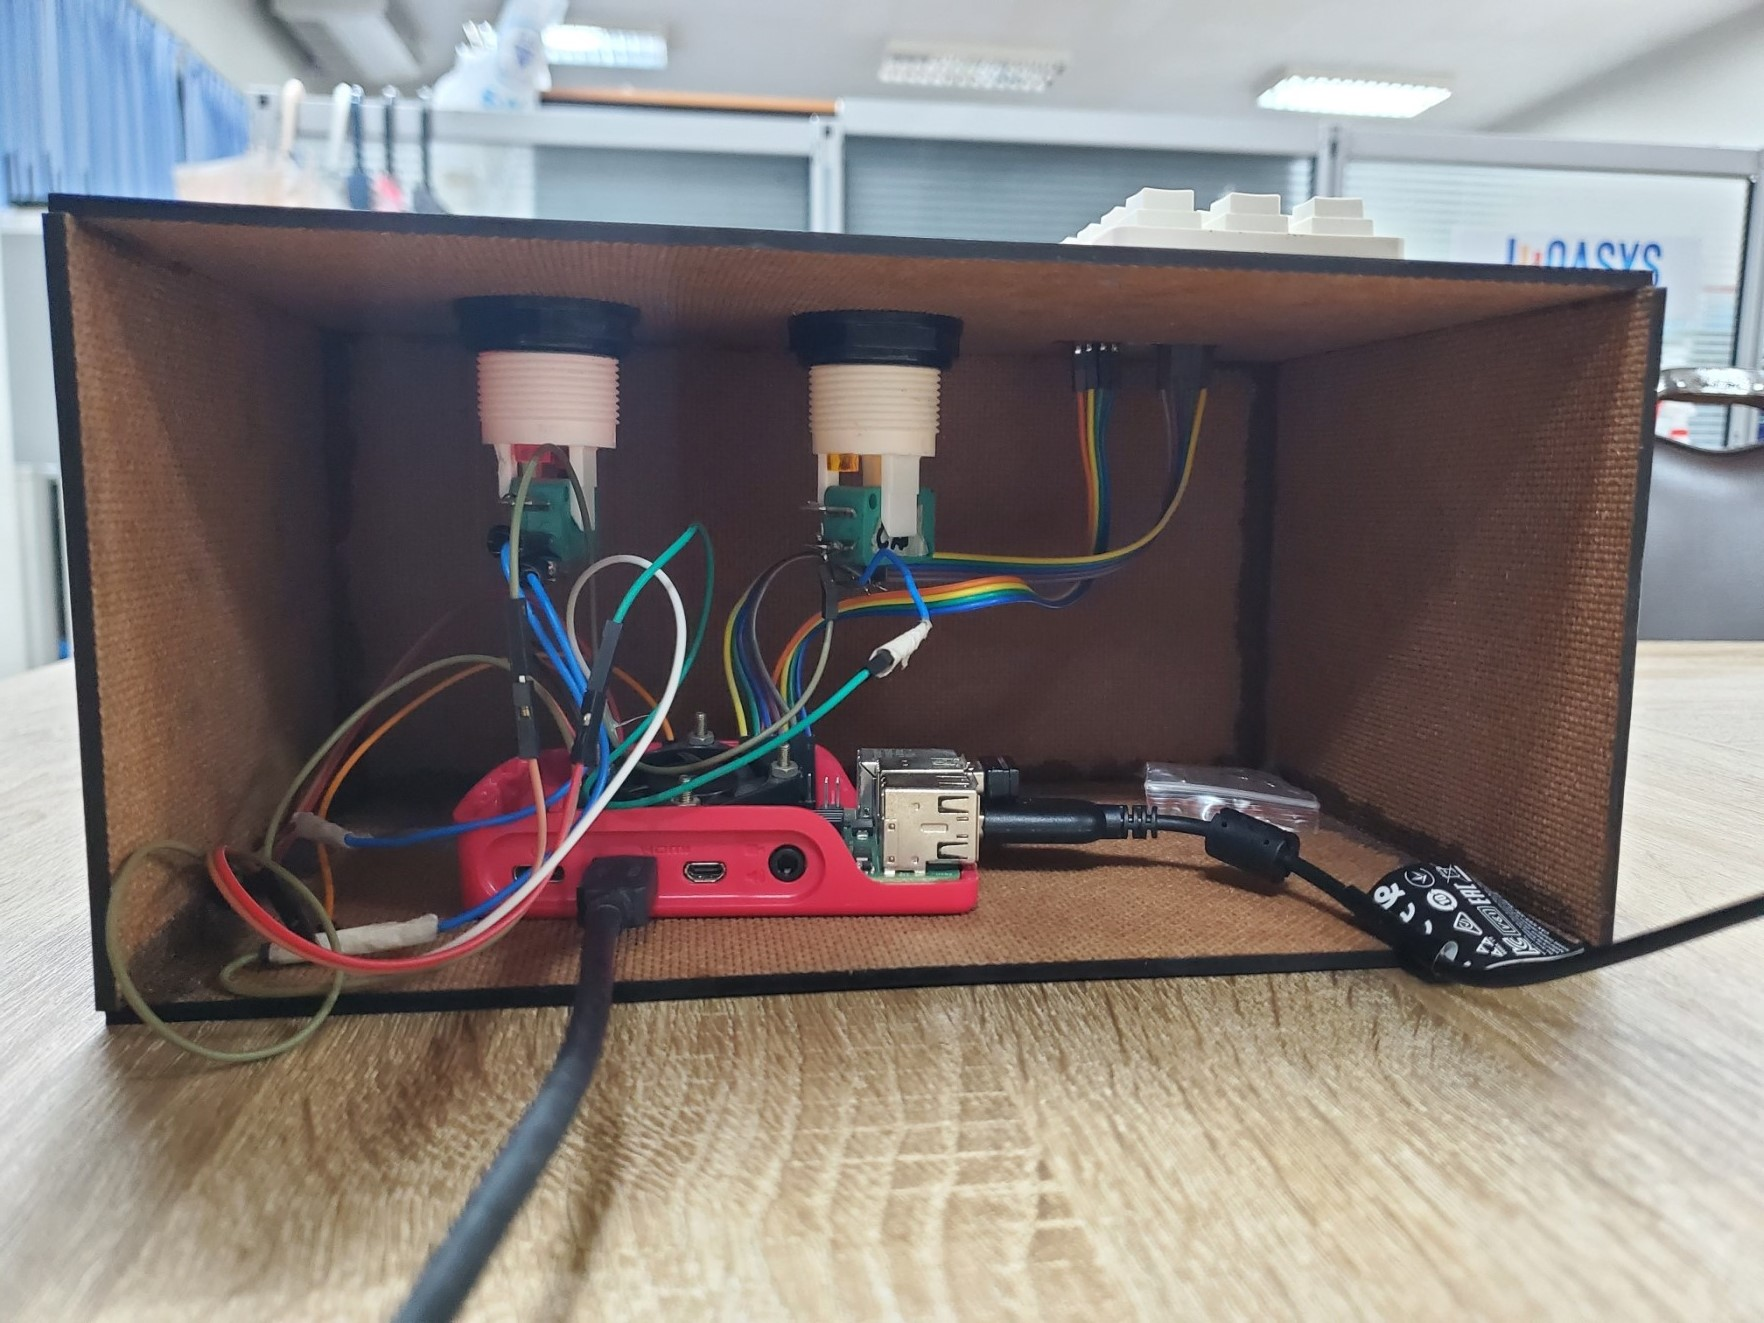
\includegraphics[scale=.17]{pic/rpi_back.jpg}
    \caption[ภายในมอดูลการตรวจจับใบหน้า และแสดงผล]{ภายในมอดูลการตรวจจับใบหน้า และแสดงผล}
    \label{fig:inside_module}
  \end{center}
\end{figure}

\begin{figure}[!ht]
  \begin{center}
    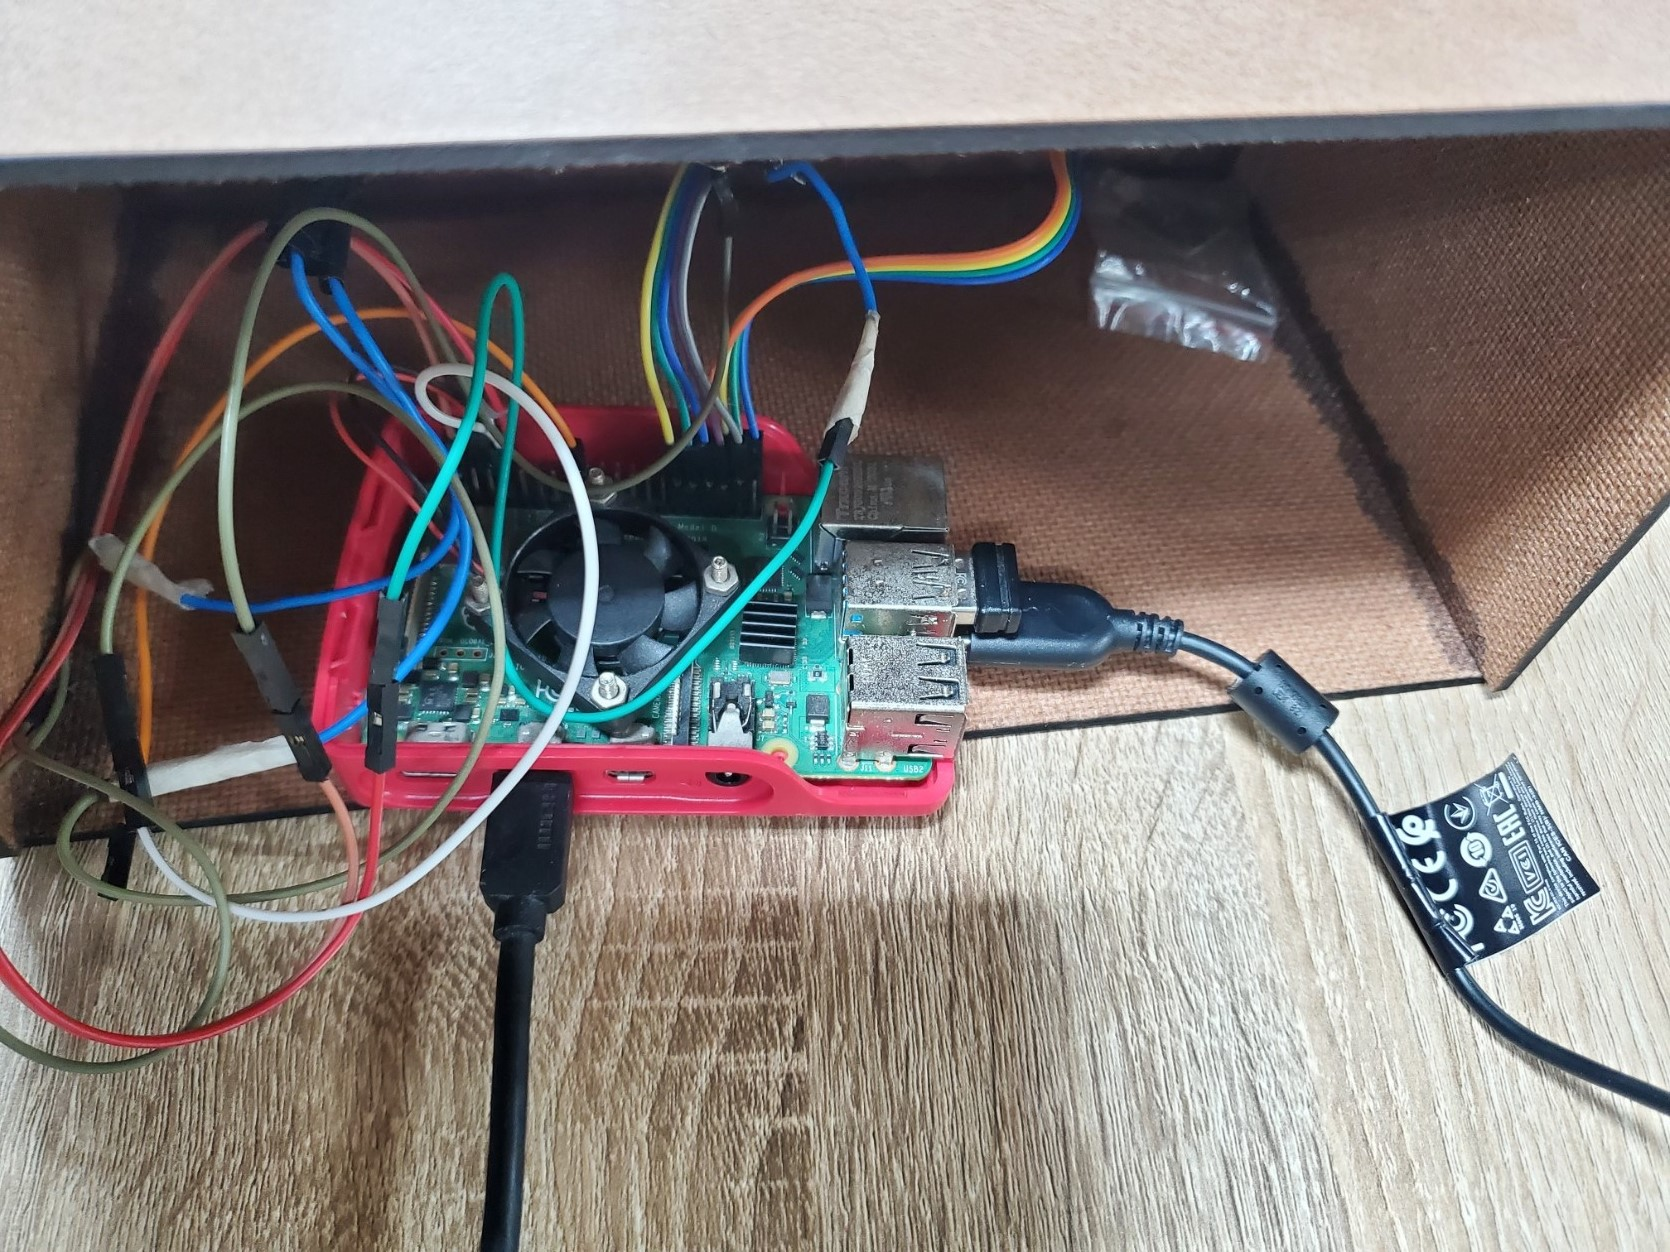
\includegraphics[scale=.17]{pic/rpi.jpg}
    \caption[การเชื่อมต่อ Raspberry Pi]{การเชื่อมต่อ Raspberry Pi}
    \label{fig:rpi_module}
  \end{center}
\end{figure}

\newpage
\section{รูปภาพการแสดงผลบนหน้าจอ}

\begin{figure}[!ht]
    \begin{center}
      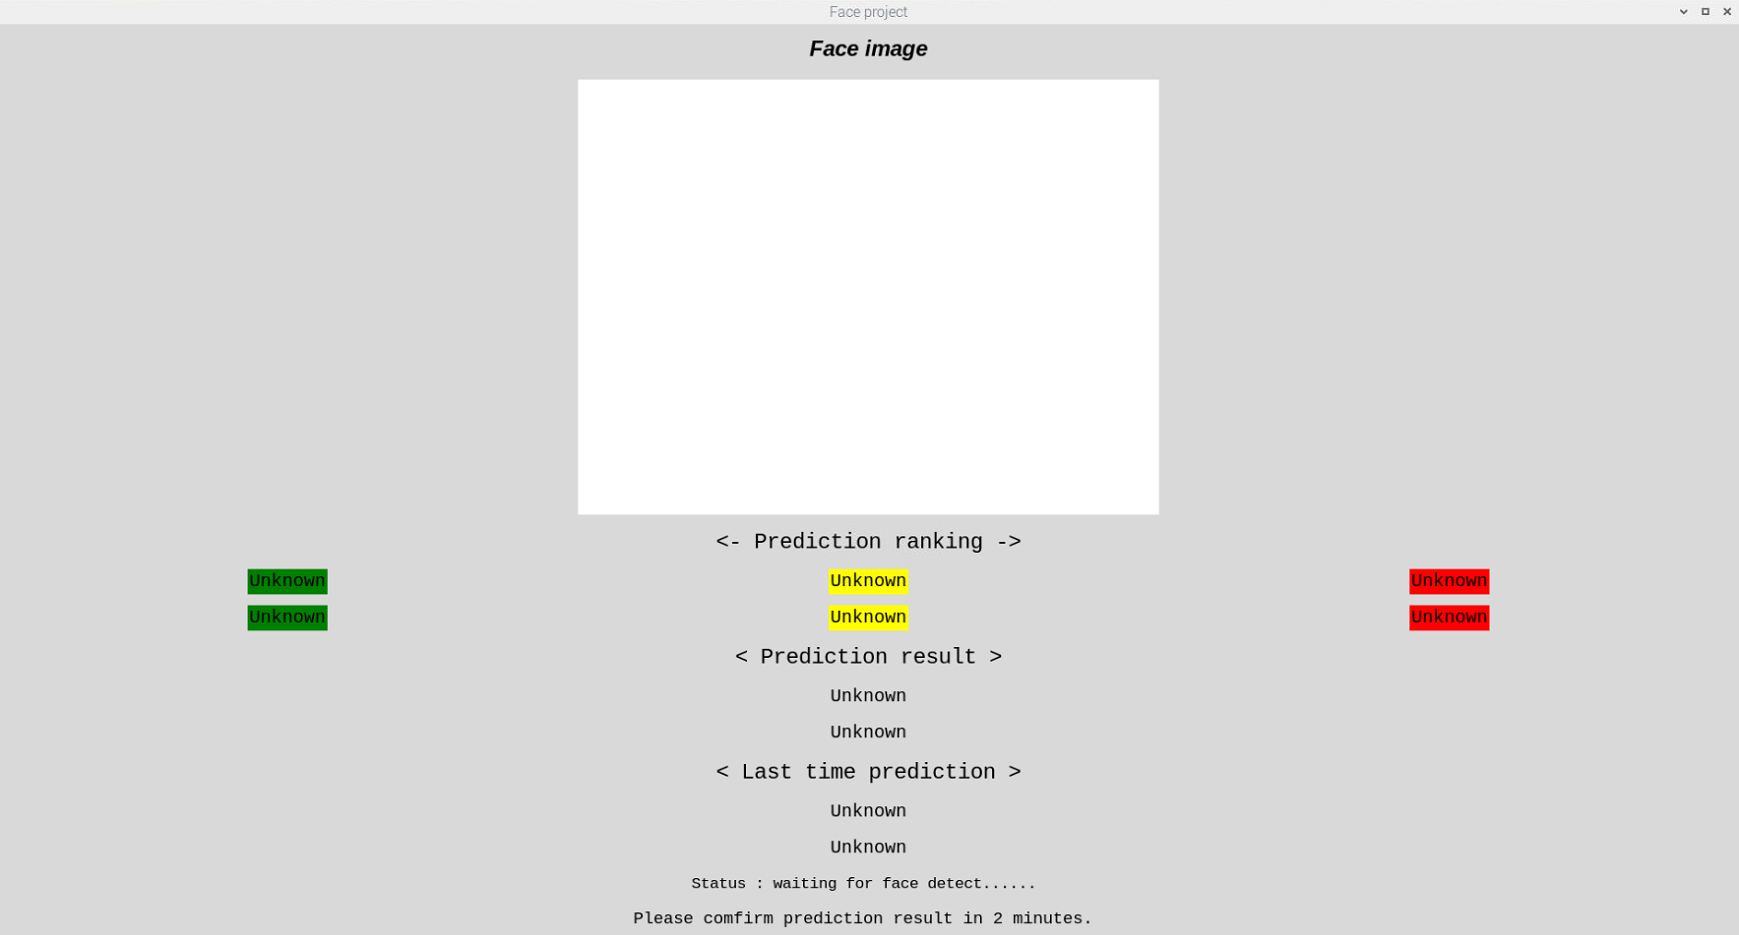
\includegraphics[scale=.35]{pic/main_page.png}
      \caption[หน้า GUI เมื่อโปรแกรมเริ่มทำงาน]{หน้า GUI เมื่อโปรแกรมเริ่มทำงาน}
      \label{fig:main_page}
    \end{center}
\end{figure}



\begin{figure}[!ht]
    \begin{center}
      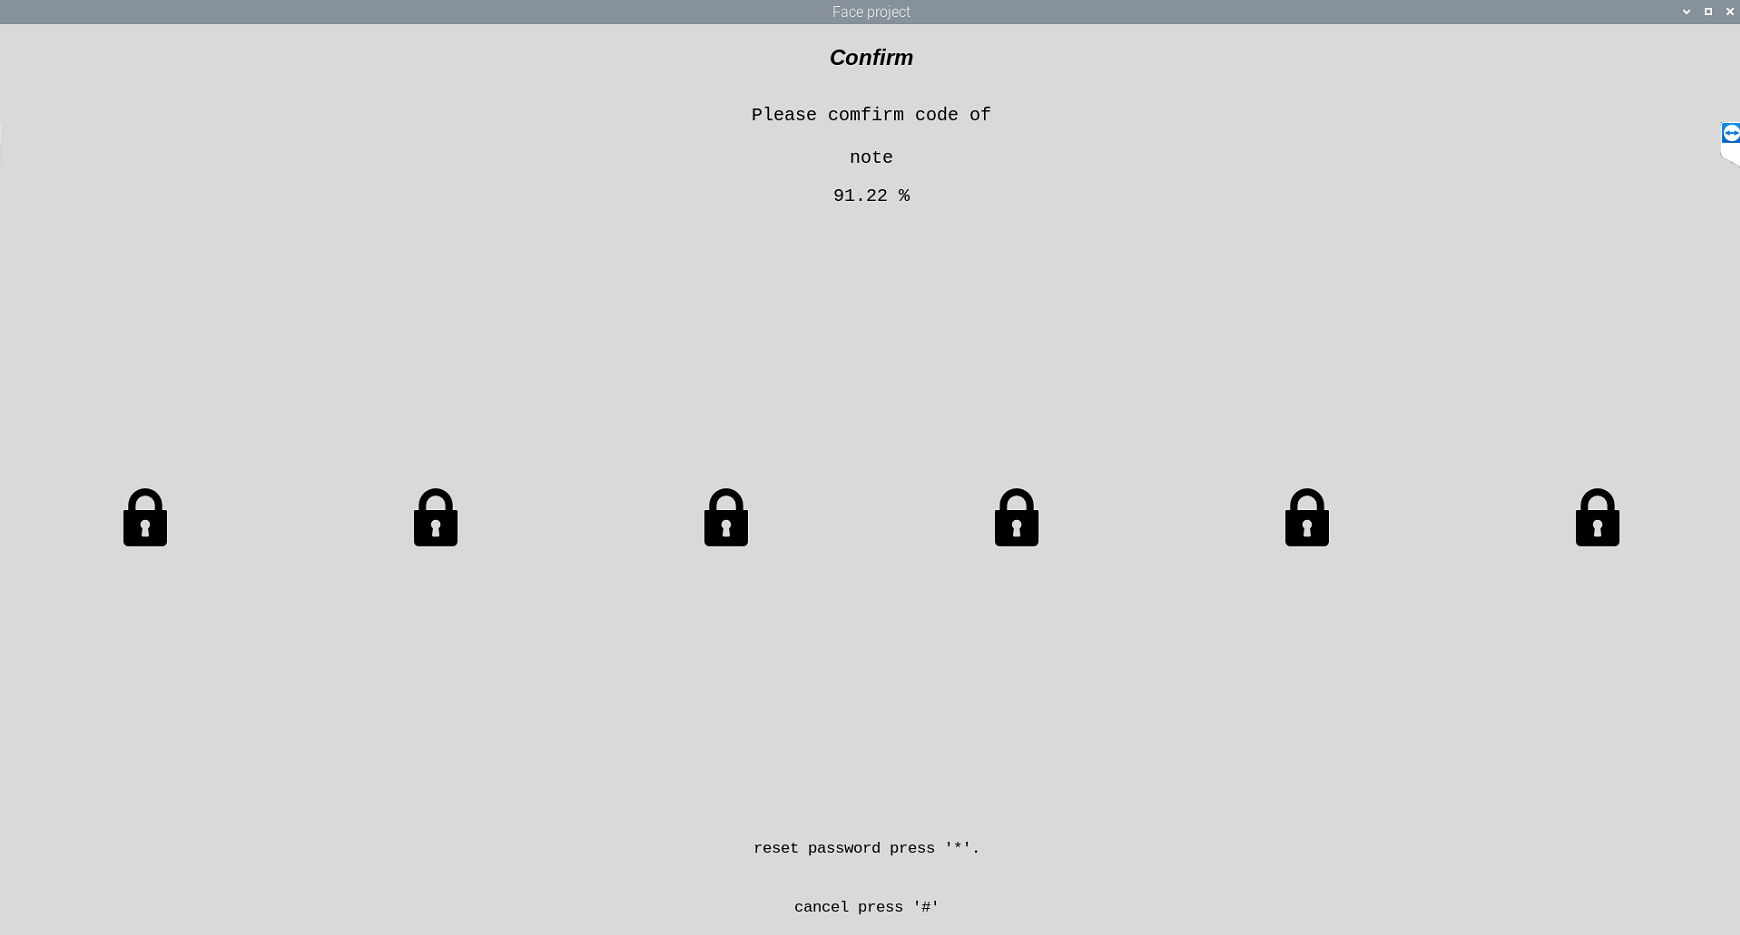
\includegraphics[scale=.35]{pic/comfirm_page.png}
      \caption[หน้า GUI เมื่อผลลัพธ์การระบุตัวตนผิด]{หน้า GUI เมื่อผลลัพธ์การระบุตัวตนผิด}
      \label{fig:com_page}
    \end{center}
\end{figure}


\begin{figure}[!ht]
  \begin{center}
    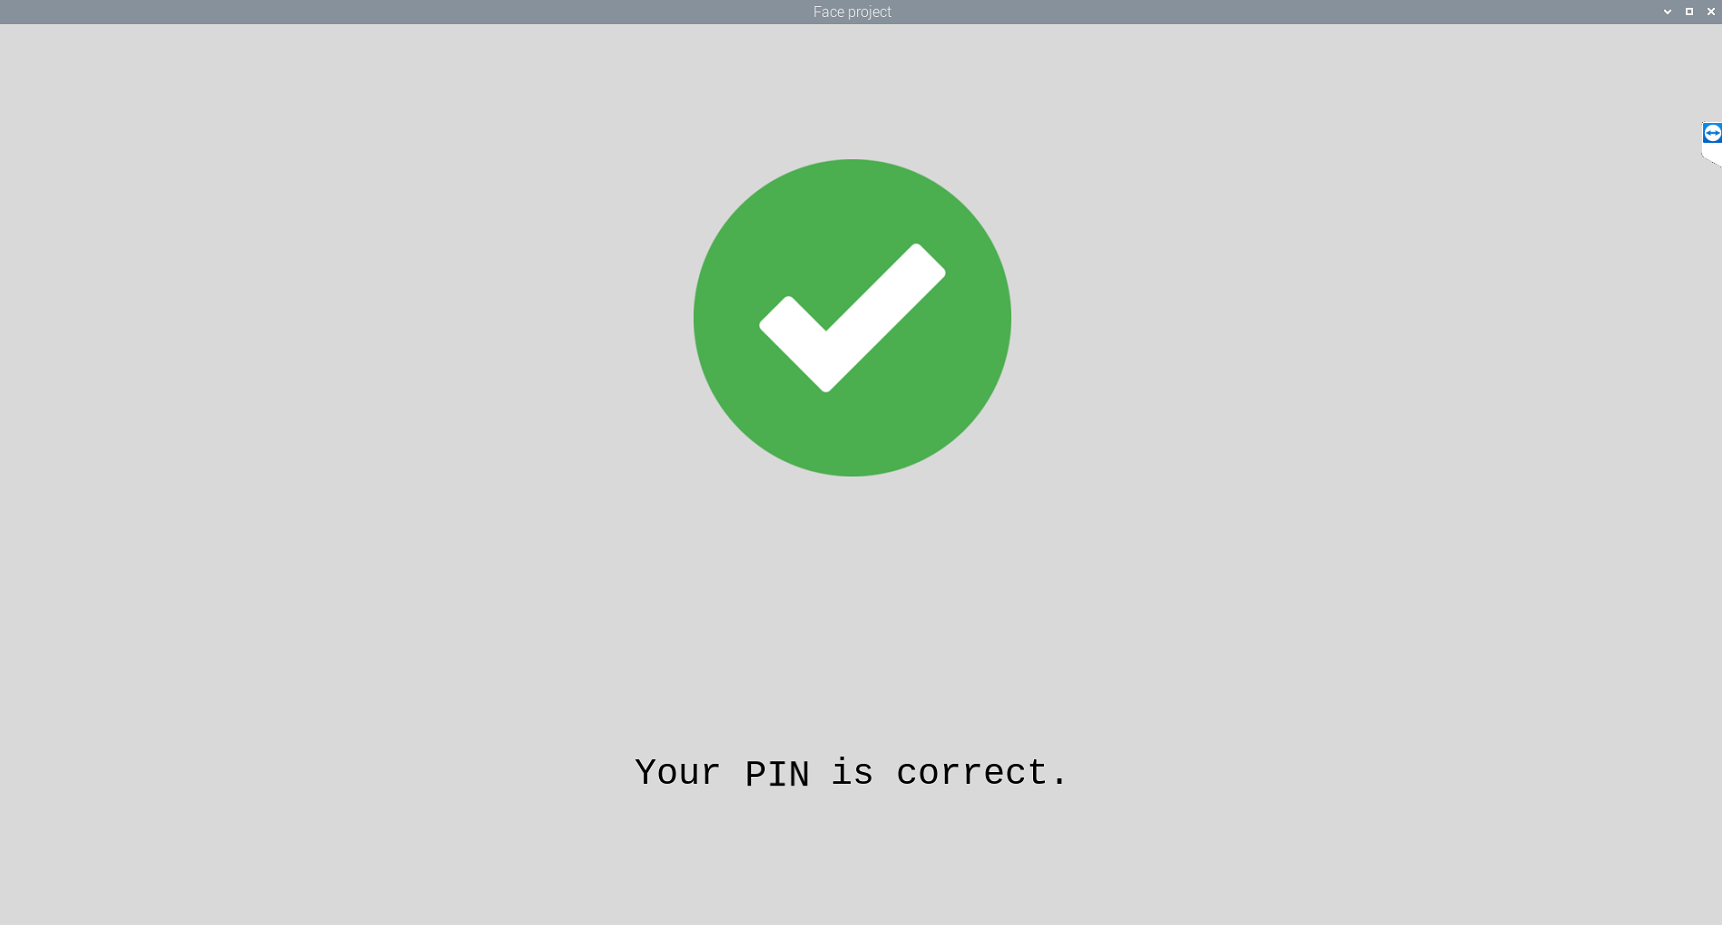
\includegraphics[scale=.35]{pic/pin_correct.png}
    \caption[หน้า GUI เมื่อผลลัพธ์รหัสยืนยันตัวตนถูกต้อง]{หน้า GUI เมื่อผลลัพธ์รหัสยืนยันตัวตนถูกต้อง}
    \label{fig:pin_correct}
  \end{center}
\end{figure}


\begin{figure}[!ht]
  \begin{center}
    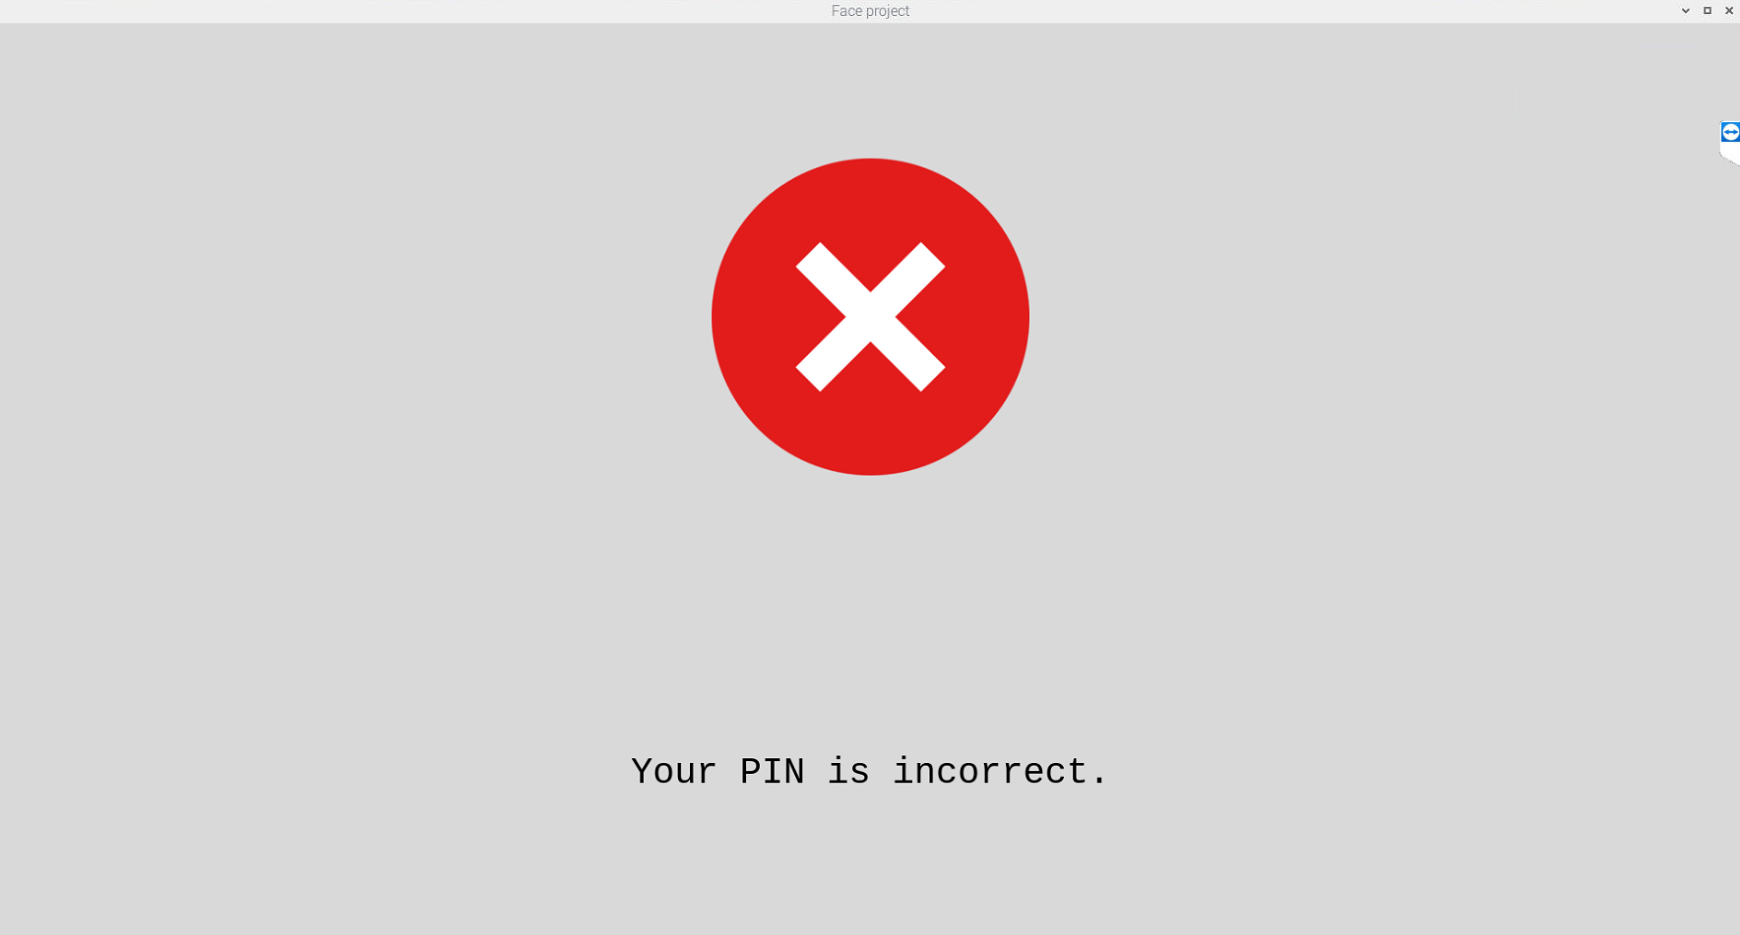
\includegraphics[scale=.35]{pic/pin_incorrect.png}
    \caption[หน้า GUI เมื่อผลลัพธ์รหัสยืนยันตัวตนไม่ถูกต้อง]{หน้า GUI เมื่อผลลัพธ์รหัสยืนยันตัวตนไม่ถูกต้อง}
    \label{fig:pin_incorrect}
  \end{center}
\end{figure}


% \textsf{test ทดสอบฟอนต์ sans serif ภาษาไทย}

% \verb+test ทดสอบฟอนต์ teletype ภาษาไทย+

% \texttt{test ทดสอบฟอนต์ teletype ภาษาไทย}

% \textbf{ตัวหนา serif ภาษาไทย \textsf{sans serif ภาษาไทย} \texttt{teletype ภาษาไทย}}

% \textit{ตัวเอียง serif ภาษาไทย \textsf{sans serif ภาษาไทย} \texttt{teletype ภาษาไทย}}

% \textbf{\textit{ตัวหนาเอียง serif ภาษาไทย \textsf{sans serif ภาษาไทย} \texttt{teletype ภาษาไทย}}}






\chapter{\ifenglish Manual\else คู่มือการใช้งานระบบ\fi}

โปรแกรมของโครงงานนี้สามารถดาวน์โหลดได้จาก \url{https://www.example.com/test_ทดสอบ_url} 
ใช้ระบบปฏิบัติการของ Raspberry Pi คือ Raspbian buster และใช้ระบบปฏิบัติการของ Windows คือ Windows 10

\section{คู่มือการติดตั้งโปรแกรมเพื่อตรวจจับใบหน้าบน Raspberry Pi}
\subsection{คู่มือการติดตั้ง OpenCV บน Raspberry Pi}
\begin{enumerate}
  \item เปิด Termenal
  \item พิมพ์คำสั่ง sudo git clone \url{https://github.com/freedomwebtech/raspbianlegacy.git}
  \item พิมพ์คำสั่ง cd raspbianlegacy
  \item พิมพ์คำสั่ง sudo chmod 775 install.sh
  \item พิมพ์คำสั่ง sudo ./install.sh จากนั้นรอจนกว่าจะเสร็จ ใช้เวลาประมาณ 2 ชั่วโมง
  \item เมื่อทำการติดตั้งเสร็จแล้วให้ทดลองใช้คำสั่ง python3
  \item แล้วพิมพ์ import cv2
  \item แล้วพิมพ์ cv2.\textunderscore\textunderscore version \textunderscore\textunderscore หากติดตั้งสำเร็จจะแสดงเลข version
\end{enumerate}

\subsection{คู่มือการติดตั้ง TensorFlow lite บน Raspberry Pi}
\begin{enumerate}
  \item เปิด Termenal
  \item พิมพ์คำสั่ง sudo git clone \url{https://github.com/freedomwebtech/raspbianlegacy.git}
  \item พิมพ์คำสั่ง cd raspbianlegacy
  \item พิมพ์คำสั่ง sudo chmod 775 tensorflow-lite.sh
  \item พิมพ์คำสั่ง sudo ./tensorflow-lite.sh จากนั้นรอจนกว่าจะเสร็จ
  \item เมื่อทำการติดตั้งเสร็จแล้วให้ทดลองใช้คำสั่ง pip show tensorflow หากติดตั้งสำเร็จจะแสดงข้อมูลของ tensorflow
\end{enumerate}

\subsection{คู่มือการติดตั้ง Mediapipe library บน Raspberry Pi}
\begin{enumerate}
  \item เปิด Termenal
  \item พิมพ์คำสั่ง sudo apt update
  \item พิมพ์คำสั่ง sudo pip3 install mediapipe-rpi4 จากนั้นรอจนกว่าจะเสร็จ
\end{enumerate}

\subsection{คู่มือการติดตั้ง Tkinter library บน Raspberry Pi}
\begin{enumerate}
  \item เปิด Termenal
  \item พิมพ์คำสั่ง sudo apt update
  \item พิมพ์คำสั่ง sudo pip3 install tk จากนั้นรอจนกว่าจะเสร็จ
\end{enumerate}


\section{คู่มือการติดตั้งโปรแกรมเพื่อระบุตัวตนใบหน้าบน Server}
\subsection{คู่มือการติดตั้ง Python บน Windows}
\begin{enumerate}
  \item ไปยังเว็บไซต์ \url{https://www.python.org/downloads/} เพื่อดาวน์โหลดตัว setup ของ Python
  \item เปิดไฟล์ setup
  \item คลิ๊ก Install Now รอจนติดตั้งเสร็จ จากนั้นสามารถกดปิดหน้าต่างการ setup ได้
  \item เมื่อติดตั้ง Python เสร็จแล้ว ให้ทดลองตรวจสอบว่า Python นั้นติดตั้งสําเร็จ โดยการเปิด cmd
  หรือ powershell แล้วใช้คําสั่ง python -V จะแสดง version ของ Python ที่ทําการติดตั้ง
\end{enumerate}

\subsection{คู่มือการติดตั้ง Flask framework}
\begin{enumerate}
  \item เปิด cmd หรือ powershell หรือ windows terminal
  \item พิมพ์คำสั่ง pip install Flask รอจนติดตั้งเสร็จ
\end{enumerate}

\subsection{คู่มือการติดตั้ง OpenCV บน Windows}
\begin{enumerate}
  \item เปิด cmd หรือ powershell หรือ windows terminal
  \item พิมพ์คำสั่ง pip install opencv-python รอจนติดตั้งเสร็จ
  \item เมื่อทำการติดตั้งเสร็จแล้วให้ทดลองใช้คำสั่ง python
  \item แล้วพิมพ์ import cv2
  \item แล้วพิมพ์ cv2.\textunderscore\textunderscore version \textunderscore\textunderscore หากติดตั้งสำเร็จจะแสดงเลข version
\end{enumerate}

\subsection{คู่มือการติดตั้ง Scikit learn บน Windows}
\begin{enumerate}
  \item เปิด cmd หรือ powershell หรือ windows terminal
  \item พิมพ์คำสั่ง pip install scikit-learn รอจนติดตั้งเสร็จ
\end{enumerate}


\section{คู่มือการใช้งานการตรวจจับใบหน้า}
\begin{enumerate}
  \item เปิด Termenal
  \item พิมพ์คำสั่ง git clone \url{https://github.com/freedomwebtech/raspbianlegacy.git}
  \item หลังจากนั้นพิมพ์คำสั่ง cd face derection
  \item เปิดไฟล์ request\textunderscore response.py 
  \item แก้ url ให้เป็นเลข IP Address ของ server รับรูปภาพ
  \item พิมพ์คำสั่ง python main\textunderscore ui.py
\end{enumerate}

หลังจากพิมพ์คำสั่ง python main\textunderscore ui.py จะแสดงหน้าตา UI ดังรูป

\begin{figure}[!ht]
  \begin{center}
    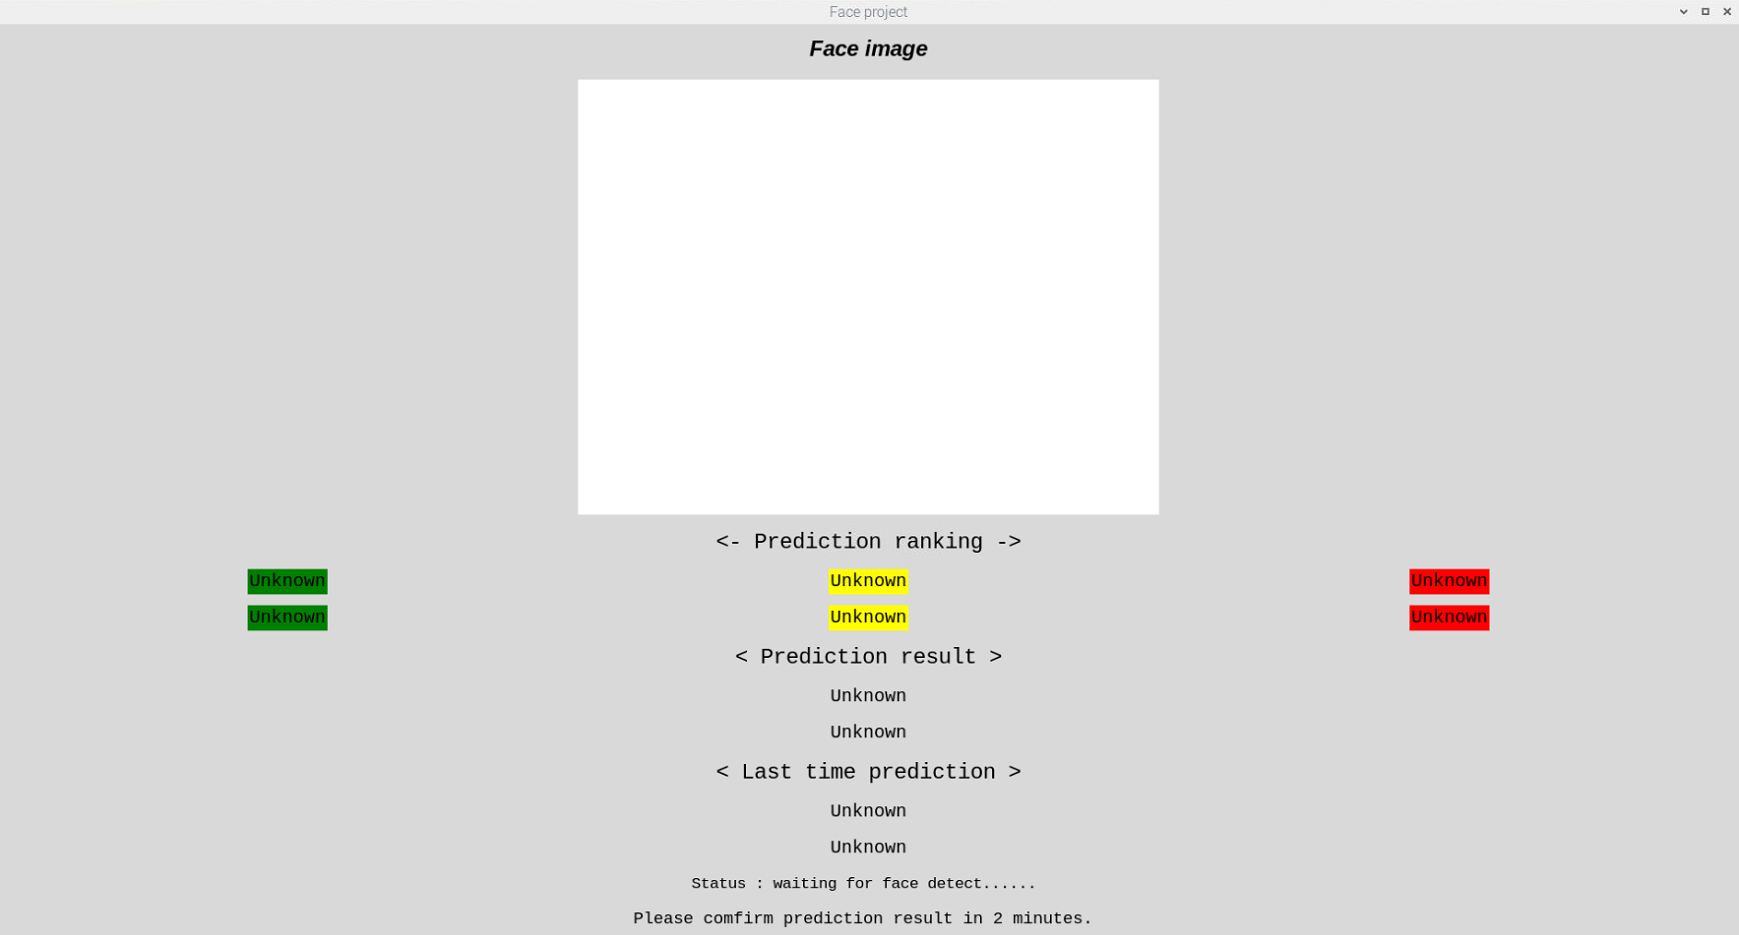
\includegraphics[scale=.3]{pic/main_page.png}
    \caption{หน้า GUI เมื่อโปรแกรมเริ่มทำงาน}
  \end{center}
\end{figure}

\section{คู่มือการใช้งานการระบุตัวตนด้วยใบหน้า}
\begin{enumerate}
  \item เปิด cmd หรือ powershell หรือ windows terminal
  \item พิมพ์คำสั่ง git clone \url{https://github.com/protonnote/backend-graduate-project.git}
  \item หลังจากนั้นพิมพ์คำสั่ง cd backend-graduate-project
  \item หลังจากนั้นเปิดไฟล์ app.py เพื่อแก้ที่จัดเก็บรูปภาพ (UPLOAD\textunderscore FOLDER) ตามเส้นทาง (path) ที่อยู่ปัจจุบันให้ถูกต้องแล้วบันทึก
  \item พิมพ์คำสั่ง python main.py
\end{enumerate}

หลังจากพิมพ์คำสั่ง python main.py จะแสดงหน้าตา Termenal ดังรูป
\begin{figure}[!ht]
  \begin{center}
    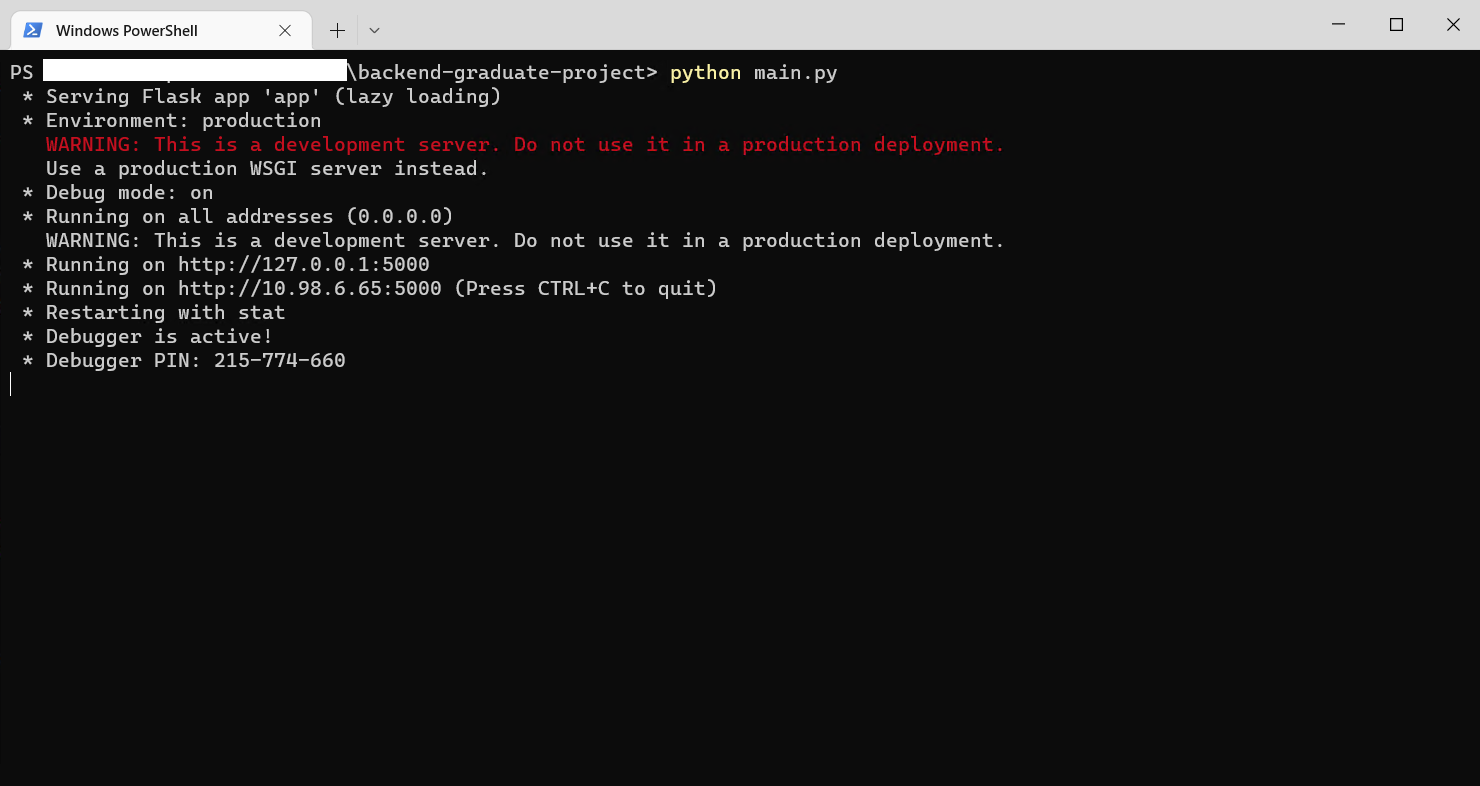
\includegraphics[scale=.4]{pic/server_start.png}
    \caption[หน้า Terminal เมื่อโปรแกรมระบุตัวตนด้วยใบหน้าเริ่มทำงาน]{หน้า Terminal เมื่อโปรแกรมระบุตัวตนด้วยใบหน้าเริ่มทำงาน}
    \label{fig:server_start}
  \end{center}
\end{figure}


\chapter{\ifenglish Manual\else เอกสารเกี่ยวกับข้อมูลส่วนบุคคล\fi}
ในโครงงานนี้ได้มีการเก็บข้อมูลส่วนบุคคลของผู้ทดลอง จึงมีหนังสือขอความยินยอม เก็บรวบรวม ใช้ และเปิดเผยข้อมูลส่วนบุคคล เพื่อนำข้อมูลรูปภาพใบหน้า 
และชื่อมาทำการเรียนรู้เพื่อสร้างแบบจำลอง (model)

\section{หนังสือขอความยินยอม เก็บรวบรวม ใช้ และเปิดเผยข้อมูลส่วนบุคคล}
\begin{figure}[!ht]
  \begin{center}
    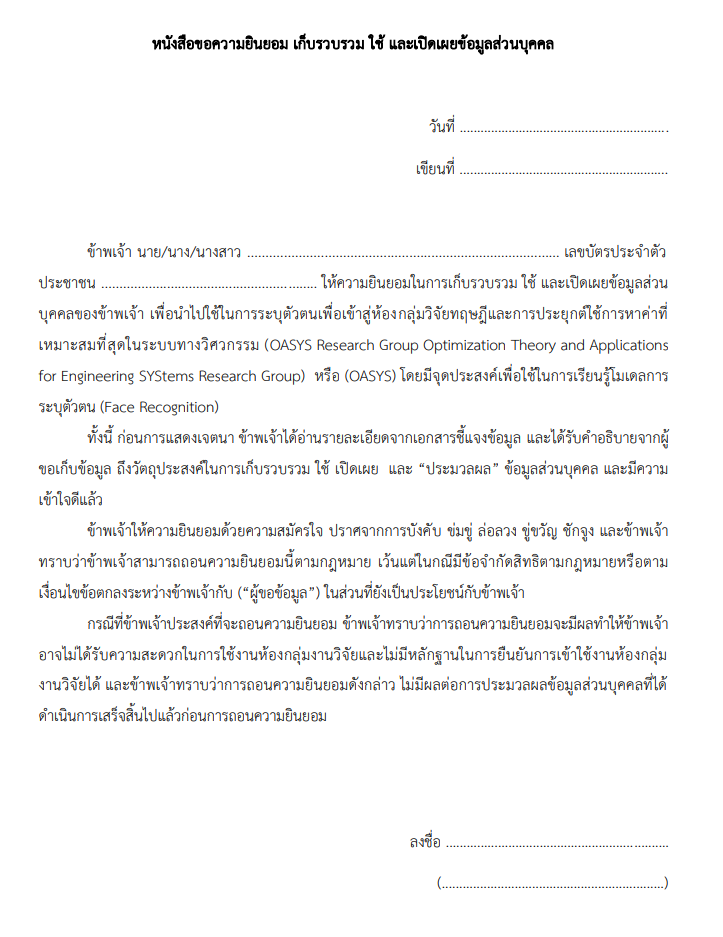
\includegraphics[scale=.85]{pic/PDPA.png}
    \caption[หนังสือขอความยินยอม เก็บรวบรวม ใช้ และเปิดเผยข้อมูลส่วนบุคคล]{หนังสือขอความยินยอม เก็บรวบรวม ใช้ และเปิดเผยข้อมูลส่วนบุคคล}
    \label{fig:pdpa}
  \end{center}
\end{figure}


%% Display glossary (optional) -- need glossary option.
\ifglossary\glossarypage\fi

%% Display index (optional) -- need idx option.
\ifindex\indexpage\fi

\begin{biosketch}
\begin{center}
  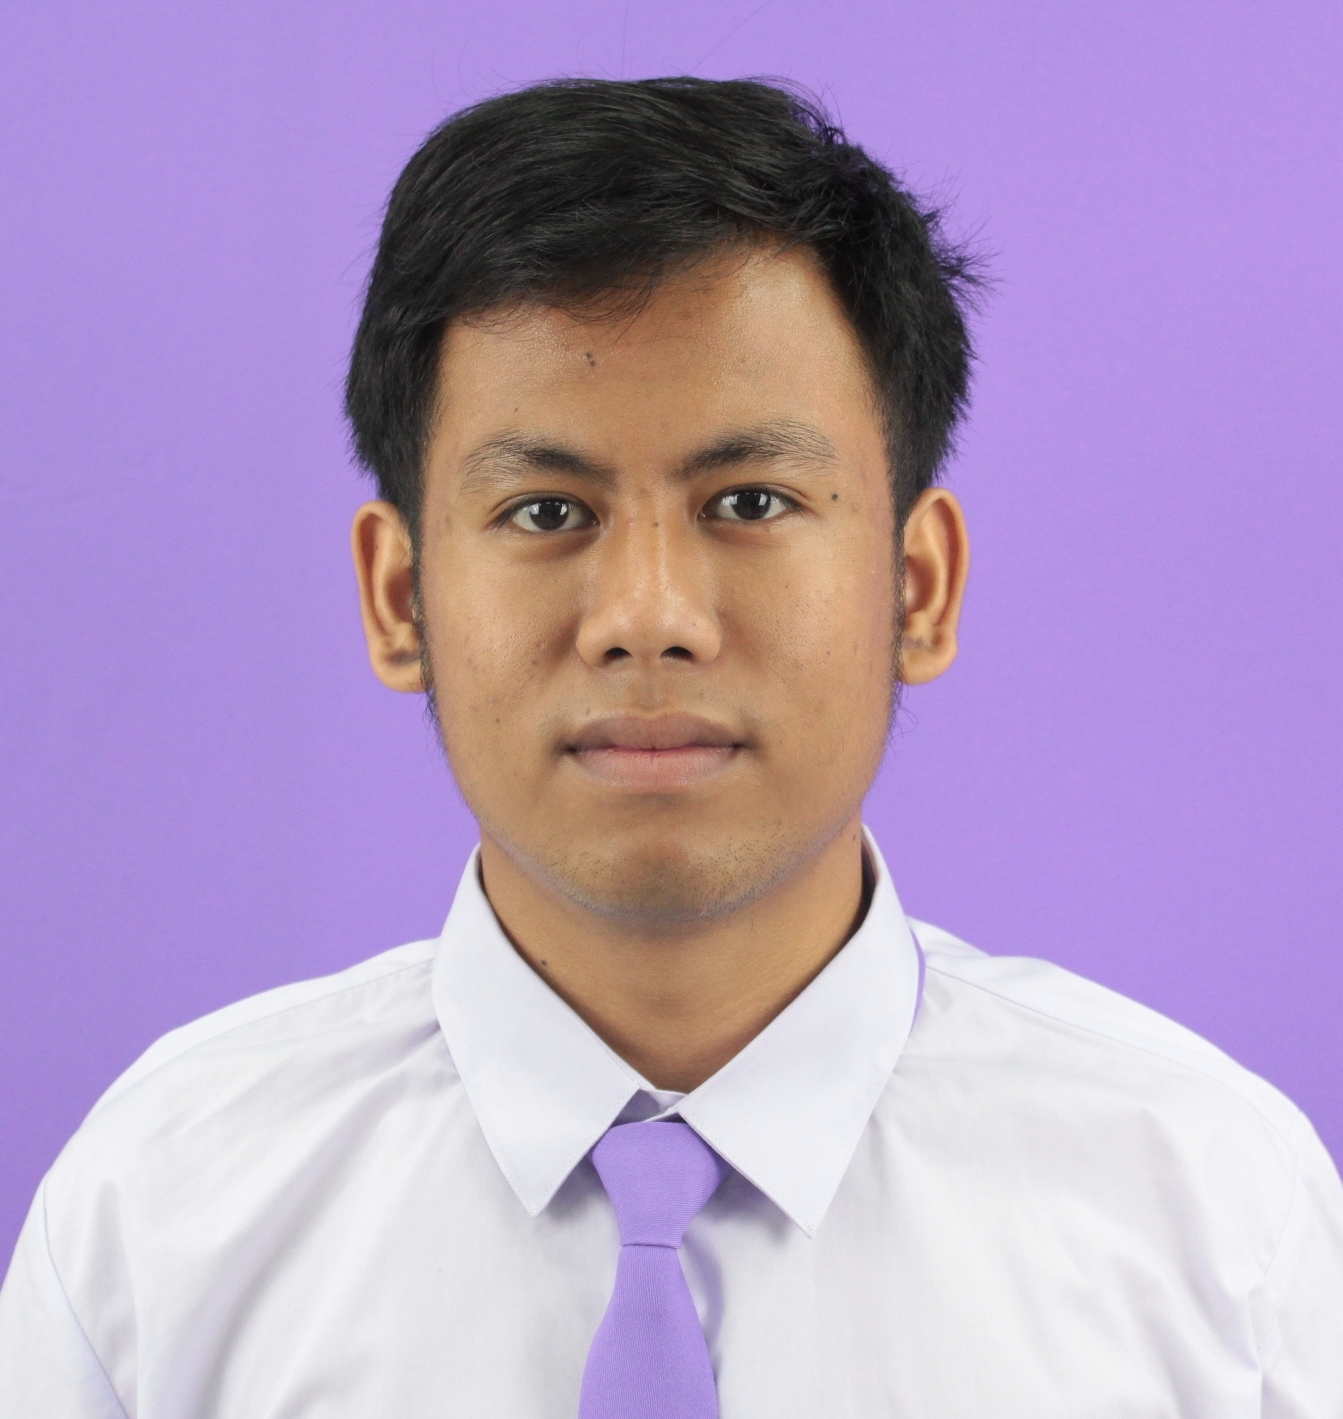
\includegraphics[width=1.5in]{pic/my_pic.jpg}
\end{center}
ชื่อ-นามสกุล : นาย นฤสรณ์ กันจินะ \\
ระดับการศึกษา : ปริญญาตรี สาขา วิศวกรรมคอมพิวเตอร์ ภาควิชา วิศวกรรมคอมพิวเตอร์ คณะ วิศวกรรมศาสตร์ มหาวิทยาลัยเชียงใหม่ \\
E-mail : naruson.kan@outlook.com \\

\textbf{กิจกรรมที่เคยเข้าร่วม}
\begin{itemize}
  \item สมาชิกทีม OASYS Data Analytics ตั้งแต่ปี พ.ศ. 2563
  \item ร่วมฝึกงานที่สำนักบริการเทคโนโลยีสารสนเทศ มหาวิทยาลัยเชียงใหม่ (Information Technology Service Center, Chiang Mai University)
\end{itemize}
% the \texttt{biosketch} environment.
\end{biosketch}
\fi % \ifproject
\end{document}
